\documentclass[11pt,a4paper]{article}
\usepackage[margin=28mm]{geometry}
\usepackage[T1]{fontenc}
\usepackage{lmodern,microtype}
\pdfgentounicode=1
\pdfglyphtounicode{tfm:lmex10/parenleftbig}{0028}
\pdfglyphtounicode{tfm:lmex10/parenrightbig}{0029}
\pdfglyphtounicode{tfm:lmex10/bracketleftbig}{005B}
\pdfglyphtounicode{tfm:lmex10/bracketrightbig}{005D}
\pdfglyphtounicode{tfm:lmex10/parenleftbigg}{0028}
\pdfglyphtounicode{tfm:lmex10/parenrightbigg}{0029}
\pdfglyphtounicode{tfm:lmex10/braceleftbigg}{007B}
\pdfglyphtounicode{tfm:lmex10/bracerightbigg}{007D}
\pdfglyphtounicode{tfm:lmex10/parenleftBigg}{0028}
\pdfglyphtounicode{tfm:lmex10/parenrightBigg}{0029}
\pdfglyphtounicode{tfm:lmex10/braceleftBigg}{007B}
\pdfglyphtounicode{tfm:lmex10/bracerightBigg}{007D}
\pdfglyphtounicode{tfm:lmex10/parenlefttp}{239B}
\pdfglyphtounicode{tfm:lmex10/parenrighttp}{239E}
\pdfglyphtounicode{tfm:lmex10/bracketlefttp}{23A1}
\pdfglyphtounicode{tfm:lmex10/bracketrighttp}{23A4}
\pdfglyphtounicode{tfm:lmex10/bracketleftbt}{23A3}
\pdfglyphtounicode{tfm:lmex10/bracketrightbt}{23A6}
\pdfglyphtounicode{tfm:lmex10/parenleftbt}{239D}
\pdfglyphtounicode{tfm:lmex10/parenrightbt}{23A0}
\pdfglyphtounicode{tfm:lmex10/summationtext}{2211}
\pdfglyphtounicode{tfm:lmex10/summationdisplay}{2211}
\pdfglyphtounicode{tfm:lmex10/productdisplay}{220F}
\pdfglyphtounicode{tfm:lmex10/integraldisplay}{222B}
\pdfglyphtounicode{tfm:lmex10/hatwide}{02C6}
\pdfglyphtounicode{tfm:lmex10/bracketleftBig}{005B}
\pdfglyphtounicode{tfm:lmex10/bracketrightBig}{005D}

\usepackage{amsmath,amssymb,amsthm,mathtools,mathrsfs,bm}
\usepackage{booktabs,graphicx,tikz}
\usetikzlibrary{arrows.meta,calc,positioning}
\usepackage[colorlinks=true,linkcolor=blue!45!black,citecolor=blue!45!black,urlcolor=blue!45!black]{hyperref}
\hypersetup{pdftitle={A directional zero-one law under strict ellipticity},pdfauthor={OpenAI}}
\pdfinfoomitdate=1
\pdftrailerid{}
\pdfsuppressptexinfo=15
\emergencystretch=2em
\newcommand{\PP}{\mathbb P}
\newcommand{\EE}{\mathbb E}
\newcommand{\ZZ}{\mathbb Z}
\newcommand{\RR}{\mathbb R}
\newcommand{\NN}{\mathbb N}
\newcommand{\1}{\mathbf 1}
\newcommand{\cF}{\mathcal F}
\newtheorem{theorem}{Theorem}[section]
\newtheorem{lemma}[theorem]{Lemma}
\newtheorem{proposition}[theorem]{Proposition}
\newtheorem{corollary}[theorem]{Corollary}
\theoremstyle{definition}
\newtheorem{definition}[theorem]{Definition}
\theoremstyle{remark}
\newtheorem{remark}[theorem]{Remark}
\title{A directional zero--one law\protect\\ under strict ellipticity}
\author{OpenAI}
\date{September 23, 2026}
\begin{document}
\maketitle
\begin{abstract}
We prove the directional zero--one conjecture for nearest-neighbor random
walks in independent and identically distributed strictly elliptic environments
on $\ZZ^d$, $d\ge3$: the probability of escape in each fixed nonzero real
direction is zero or one. Only strict positivity of the transition probabilities
is required; no uniform lower bound or moment assumption is imposed.
\end{abstract}
{\small
\tableofcontents
\par}
\section{Introduction}\label{sec:introduction}

A walk in a fixed environment is a Markov chain. Averaging over an
independent environment at every lattice site creates a different
process: revisiting a site also revisits information about its transition
probabilities. The directional zero--one problem asks whether the
annealed probability of escape in one prescribed direction can lie
strictly between zero and one. We resolve this problem positively in
every dimension $d\ge3$ for iid nearest-neighbor environments with
strictly positive transition probabilities. No common positive lower
bound on those probabilities is assumed.

\subsection{The model and the theorem}

Let $d\ge3$ be an integer, let $e_1,\ldots,e_d$ be the coordinate basis,
and set
\[
 U=\{\pm e_1,\ldots,\pm e_d\},\qquad
 \mathcal P_U=\left\{p\in[0,1]^U:\sum_{e\in U}p(e)=1\right\},
 \qquad \Omega=\mathcal P_U^{\ZZ^d}.
\]
Equip $\Omega$ with its product Borel $\sigma$-field.
An environment $\omega\in\Omega$ assigns a transition vector
$\omega(x,\cdot)$ to each site $x$. We call this vector the \emph{row}
at $x$. Let $\mu$ be a probability measure on $\mathcal P_U$, and let
$\PP=\mu^{\otimes\ZZ^d}$. Thus the rows are independent and identically
distributed; entries within one row need not be independent. Assume only
\begin{equation}\label{eq:ellipticity}
 \mu\bigl(\{p\in\mathcal P_U:p(e)>0\text{ for every }e\in U\}\bigr)=1.
\end{equation}
We call this \emph{strict ellipticity}. By countability, it gives
$\omega(x,e)>0$ simultaneously for all sites and steps, almost surely.
Unlike uniform ellipticity, it permits the smallest row entry to be
arbitrarily close to zero.

The path space is $\mathcal X=(\ZZ^d)^{\NN_0}$ with coordinate
maps $X_n$ and the $\sigma$-field $\sigma(X_n:n\ge0)$. For $x\in\ZZ^d$ and a fixed environment, the
\emph{quenched law} $P_{x,\omega}$ is the Markov-chain law specified by
\[
 P_{x,\omega}(X_0=x)=1,\qquad
 P_{x,\omega}(X_{n+1}=X_n+e\mid X_0,\ldots,X_n)=\omega(X_n,e).
\]
The \emph{annealed law} and its expectation are
\[
 P_x(B)=\int P_{x,\omega}(B)\,\PP(d\omega),\qquad E_x.
\]
When both environment and path are needed, we use the joint law
$\mathsf P_x(d\omega,dX)=\PP(d\omega)P_{x,\omega}(dX)$.
The path filtration is $\mathcal F_n=\sigma(X_0,\ldots,X_n)$;
on the joint space the larger filtration
$\mathcal G_n=\sigma(\omega,X_0,\ldots,X_n)$ also reveals the entire
environment. Quenched Markov arguments use $\mathcal G_n$.
The endpoint-posterior martingales later in the proof use
$\mathcal F_n$, with the environment integrated out.
An unconditioned annealed path law will also be called the \emph{raw law}.

For a nonzero vector $\ell\in\RR^d$, define
\[
 A_\ell=\{X_n\cdot\ell\longrightarrow+\infty\}.
\]
\begin{theorem}\label{thm:main}
Let $d\ge3$, let $\PP$ be an independent and identically distributed
law of nearest-neighbor transition rows on $\ZZ^d$ satisfying
\eqref{eq:ellipticity}, and let $\ell\in\RR^d\setminus\{0\}$.
Then
\[
 P_0(A_\ell)\in\{0,1\}.
\]
\end{theorem}

The direction is any fixed real vector; no rationality assumption is
made, and no assertion of one exceptional null set uniform over all
directions is needed. No inverse-transition or logarithmic moment,
drift, balance, reversibility, or speed condition supplements
\eqref{eq:ellipticity}. In the proof, a finite first moment for a
\emph{spatial radius} is derived under the hypothesis that both signs
have positive probability. No first moment for a regeneration duration,
positive speed or ballisticity assertion is used or obtained from that
estimate.

\subsection{Prior work}

The directional question goes back to Kalikow~\cite{Kalikow1981};
see also the historical discussion in~\cite{Zerner2007}.
The classical sign-union zero--one law concerns
$P_0(A_\ell\cup A_{-\ell})$, not $P_0(A_\ell)$.
It originates in the uniformly elliptic theory of
Kalikow~\cite{Kalikow1981}; its strict-ellipticity extension is
\cite[Proposition~3]{ZernerMerkl2001}, as recalled in
\cite[Equation~(1)]{Zerner2007}. Zerner and Merkl proved the
one-sign directional law in dimension two for iid strictly elliptic
environments~\cite[Theorem~1]{ZernerMerkl2001}, and Zerner gave a shorter
proof~\cite{Zerner2007}. Slonim extended the planar iid law to bounded jumps
when almost surely there is a unique infinite communicating class reachable
from every site~\cite[Theorem~2.1]{Slonim2024}. Theorem~\ref{thm:main} establishes
the directional zero--one conjecture for nearest-neighbor walks in every
higher dimension under strict ellipticity.

The difficulty in higher dimensions is that the planar arguments force
oppositely directed paths to meet by geometry; their quantitative
counterpart must be supplied differently here. Berger proved that in
dimensions $d\ge5$ an iid uniformly elliptic walk has at most one nonzero
limiting velocity~\cite[Theorem~1.1]{Berger2008}. This allows a second
velocity equal to zero and leaves open the possibility of opposite
directional escape at zero speed. Independence is also substantive:
Bramson, Zeitouni, and Zerner constructed stationary, polynomially mixing,
uniformly elliptic environments in $d\ge3$ with positive probabilities of
linear escape in opposite directions~\cite[Theorem~3]{BramsonZeitouniZerner2006}.
Their Open Problem~3 formulates the higher-dimensional question for iid
uniformly elliptic environments.

A non-uniformly elliptic special case is provided by Dirichlet-distributed
rows. Sabot and Tournier obtained positive-probability transience in coordinate
directions with positive corresponding mean drift, using reversal identities
specific to that distribution~\cite[Theorem~1]{SabotTournier2011}.
Bouchet proved the fixed-direction zero--one law in this class for $d\ge3$
by studying an accelerated walk and an invariant law for the environment
viewed from the particle~\cite[Corollary~4]{Bouchet2013}. Tournier identified
the asymptotic direction as that of the initial drift when this drift is
nonzero~\cite[Corollary~1]{Tournier2015}. The argument below applies to arbitrary iid
strictly positive rows and uses only translations of its path pieces.

The regeneration structure of Sznitman and Zerner~\cite{SznitmanZerner1999}
is a central tool. We give the factorization and width arguments needed
below, including the distinction between real projected heights and
integer record indices. Simenhaus proved that distinct deterministic
asymptotic directions occurring with positive probability must be
opposite~\cite[Proposition~1]{Simenhaus2007}. His existence theorem for
an asymptotic direction assumes transience on a nonempty open set of
directions. Drewitz and Ram\'{i}rez obtained a corresponding two-ray
description under sign-union transience on an open set, equivalently in
$d$ linearly independent directions~\cite[Theorem~1.8]{DrewitzRamirez2010}.
Those hypotheses do not follow here from the initial assumption in one
direction. In our contradiction argument, the spatial radius estimate
supplies the two rays first; a self-contained argument then proves
their antipodality. The remaining estimates concern contacts between
two arrangements of regeneration pieces.

\subsection{Proof strategy}

Two fresh-row arguments make the proof work without a common positive
lower bound on the transition probabilities. First, finite-width slab escape
(Lemma~\ref{lem:finite-supremum}) is
proved using recurrent-site trials and first visits to new columns,
in the spirit of \cite[Lemma~4]{ZernerMerkl2001}. Second, scripts launched
from a tilted record use pairwise distinct, previously unused rows.
Their annealed cost is a product of positive row averages, rather than
a product of uniform quenched lower bounds.

Suppose, toward a contradiction, that $0<P_0(A_\ell)<1$.
A slab-exit argument and fresh-half-space regeneration first show that
the path escapes in one of the two signs almost surely.
At a strict record from which the path
never falls below its new height, the future factors from the past.
The path between successive such records is a finite \emph{regeneration
piece}. Under conditioning never to backtrack, these pieces are
independent and identically distributed. Their mean height width is
finite, even for an irrational direction.

The first main step, Proposition~\ref{prop:radius}, proves that
coexistence of the two signs also forces finite mean spatial radius of
a piece. A very large lateral
excursion would create a record in a tilted direction. From that record,
a fresh continuation escaping in the opposite sign has a probability
bounded below independently of the excursion scale. This would give a
fixed positive probability to arbitrarily large finite height maxima,
contradicting the tail of their distribution.
The radius bound gives deterministic limiting rays on the two escape
events; the rays must be opposite. We may therefore reduce to
coexistence in one coordinate direction.

We then sample two independent sequences of coordinate regeneration
pieces. Place positive pieces downward by successively anchoring their
\emph{terminal} points, and place negative pieces downward in their
ordinary chronological order. Individual path words retain their
original orientation. Heights at which both sequences have a piece
boundary divide the arrangement into independent common blocks.
A \emph{contact} is a site from which both arranged paths depart.
For each dyadic interval of common-block indices, consider whether a
contact occurs. Let $m(J)$ be the sum of these probabilities over the
first $J$ such intervals, as defined precisely in
\eqref{eq:contact-count}.

The two final steps give
\[
 m(J)=O\!\left(\frac{J}{\log J}\right),\qquad
 m(J)\ge c\,\frac{J}{\log\log J}\quad\text{for large }J,
\]
with $c>0$, which are incompatible.
For the upper bound, Proposition~\ref{prop:entropy-upper} compares the
arrangement with independent bridges of prescribed heights. Randomizing
the number of blocks keeps the cost of replacing each chunk by bridges
of its realized height bounded.
An independent stretch of blocks before the comparison interval turns the
lateral alignment cost into an increment of displacement entropy. These
increments telescope over dyadic scales, while finite mean widths make
the bridge contact probabilities summable on those scales. A
relative-entropy bound converts these two estimates into the stated bound
for the expected number of contact intervals.

For the lower bound, view a positive bridge in chronological order and
start the negative path just below its random endpoint. A union bound
over all possible endpoints would be too expensive. Instead, the
conditional probabilities of the possible endpoints form a vector of
annealed martingales. Lemma~\ref{lem:posterior-maxima} bounds the sum of
their running maxima by an exponential tail on a logarithmic scale.
In Proposition~\ref{prop:contact-bound}, first-contact prefixes are transferred to
one shared environment before they are classified by quenched exit
probabilities; the posterior functions remain in the unrevealed
annealed path filtration. This separation controls the endpoint-dependent
alignment without imposing a martingale property after the environment
is revealed. A range of dyadic height intervals without a contact forces
a late first contact near the top. Applying the estimate at the many
regeneration boundaries in that range yields many contact height scales.
The finite mean common-block width then converts the height
count into the block-index count $m(J)$.

Section~\ref{sec:regeneration} proves the path-weight and regeneration
facts. Section~\ref{sec:radius} establishes the spatial moment bound.
Section~\ref{sec:arrangement} reduces to coordinate heights and defines
the common arrangement. Sections~\ref{sec:entropy} and
\ref{sec:posterior} prove the entropy and endpoint-posterior estimates.
Section~\ref{sec:contradiction} gives the lower contact count and
completes the theorem.

\section{Regeneration in a real direction}\label{sec:regeneration}

Following the regeneration approach of Sznitman and
Zerner~\cite{SznitmanZerner1999}, we construct finite path pieces whose
successive translates are independent.  Their terminal times are selected using the entire future, so the usual
stopping-time Markov property does not establish this independence.  An exact
factorization of finite path weights will do so.  Counting ordinary records
then gives a finite mean projected width, even when the projected heights do
not lie in a discrete subgroup of $\RR$.

\subsection{Departure rows and path weights}

A finite nearest-neighbor word is a sequence
$\gamma=(x_0,\ldots,x_m)$ with $x_{j+1}-x_j\in U$.  Its departure set and
annealed weight are
\[
 \operatorname{Dep}(\gamma)=\{x_0,\ldots,x_{m-1}\},\qquad
 W(\gamma)=\EE\!\left[
       \prod_{j=0}^{m-1}\omega(x_j,x_{j+1}-x_j)\right],
\]
where the expectation in this display is over the environment.  Thus
$W(\gamma)=P_{x_0}(X_j=x_j,\ 0\le j\le m)$.  A row visited repeatedly
contributes repeatedly to the same product inside the expectation.  The
terminal site contributes no row unless the word departed from it earlier.
Translation invariance gives $W(\gamma+z)=W(\gamma)$.

\begin{lemma}[Transfer through unused departure rows]
\label{lem:departure-transfer}
Let $\gamma=(x_0,\ldots,x_m)$ be a finite nearest-neighbor word and let
$f(\omega)$ be a nonnegative measurable function of the rows outside
$\operatorname{Dep}(\gamma)$.  Then
\begin{equation}\label{eq:departure-transfer}
 \EE\!\left[
   \prod_{j=0}^{m-1}\omega(x_j,x_{j+1}-x_j)f(\omega)\right]
       =W(\gamma)\EE[f].
\end{equation}
In particular, two prescribed words with disjoint departure sets have the
same joint weight when sampled under independent annealed laws as when
sampled independently conditional on one shared environment.

The identity also applies when $f(\omega)$ is the quenched probability of an
event for another walk stopped on its first arrival in
$\operatorname{Dep}(\gamma)$.  Events that require this other walk to avoid
that set forever are allowed.
\end{lemma}

\begin{proof}
The product in \eqref{eq:departure-transfer} depends only on rows in
$\operatorname{Dep}(\gamma)$, which are independent of all the rows defining
$f$.  This proves the identity.  For two words, conditional independence in
the shared environment gives the product of their quenched weights, and
\eqref{eq:departure-transfer} factors its environment expectation.

A trajectory stopped on arrival in a set does not use the row at that
arrival site.  Its finite stopped-prefix probabilities therefore depend
only on rows outside the set.  The same is true of every measurable event
of the stopped trajectory, by the monotone class theorem.  This includes
events on which the stopping time is infinite.
\end{proof}

The transfer is made for unclassified path weights.  A condition involving
a quenched exit probability can depend on rows on both sides of the
separation and cannot simply be inserted into the independent side of
\eqref{eq:departure-transfer}.  Later we will first apply this identity and
then classify sites in the shared environment.

\subsection{Fresh records and true cuts}

Fix $v\in\RR^d\setminus\{0\}$, normalized by $\|v\|_\infty=1$, and write
$h(x)=x\cdot v$.  Define
\[
 D_v=\{h(X_n)\ge0\text{ for all }n\ge0\},\qquad
 p_v=P_0(D_v),\qquad
 \widehat P_v=P_0(\,\cdot\mid D_v)
\]
when $p_v>0$.  All statements in Section~\ref{sec:regeneration} concern this fixed real
direction.  We write $\widehat E_v$ for expectation under
$\widehat P_v$.  No arithmetic assumption on the coordinates of $v$ is
imposed.

The next lemma follows the repeated-trial approach of Zerner and
Merkl~\cite[Lemma~4]{ZernerMerkl2001}. We give the argument to specify
which transition rows remain unused at each trial.

\begin{lemma}[Finite height supremum]\label{lem:finite-supremum}
For this fixed real direction, almost surely under $P_0$,
\[
 \sup_{n\ge0}h(X_n)<\infty
 \quad\Longrightarrow\quad h(X_n)\longrightarrow-\infty.
\]
In particular, a finite height interval cannot contain the path forever.
The corresponding statements hold from every translated starting site,
and hold quenched for almost every environment, simultaneously for all
such starting sites.
\end{lemma}

\begin{proof}
Fix nonnegative integers $b,k$, a signed coordinate step $a\in U$ with
$h(a)=1$, and an integer $m>b+k$.  It suffices to rule out
\[
 E_{b,k}=\{h(X_n)\le b\text{ for every }n,
                  \ h(X_n)\ge-k\text{ infinitely often}\}.
\]
Partition the lattice into columns, the cosets of $\ZZ a$.  Every column
has only finitely many sites with height in $[-k,b]$: its successive
heights differ by exactly one, regardless of the other coordinates of
$v$.

First suppose that only finitely many columns are visited at heights at
least $-k$.  On $E_{b,k}$, some fixed site $x$ of height in $[-k,b]$ is
then visited infinitely often.  Fix an environment whose transition
entries are all positive.  At every visit to this particular site the
quenched probability of the script consisting of $m$ steps $a$ is
\[
 q_x(\omega)=\prod_{j=0}^{m-1}\omega(x+ja,a)>0.
\]
Choose the first visit as a trial start, and subsequently choose the
first visit at least $m$ steps after the preceding start.  These are
stopping times.  By the quenched strong Markov property, the probability
that $r$ such trials are finite and all fail is at most
$(1-q_x(\omega))^r$.  Infinitely many visits provide infinitely many
trials, while a successful script would cross above $b$.  Thus the
specified event has quenched probability zero.  A countable union over
$x$ and integration over the environment handle this first case.  There
is no need to bound $q_x(\omega)$ uniformly in $x$ or $\omega$.

For the other case, consider the first visit, for each column, to its
portion of height at least $-k$.  These eligibility decisions are
determined by the observed path prefix.  Select the first eligible time
as a trial start, and thereafter the first eligible time at least $m$
steps after the preceding trial start.  If infinitely many columns have
such visits, infinitely many trial starts remain after these finite
exclusions.  At an eligible time, every earlier visit in the same
column had height below $-k$.  Consequently the $m$ scripted departure
sites, all at height at least $-k$, are distinct and have not appeared
earlier.  Conditional on any fixed eligible prefix, their rows retain
their original independent laws.  The annealed conditional probability
of the script is therefore exactly
\[
 q_a^m,\qquad q_a:=\EE[\omega(0,a)]>0.
\]
The probability that $r$ selected trials are finite and all fail is at
most $(1-q_a^m)^r$.  On $E_{b,k}$ every one fails, so the second case is
also null.  This argument uses no conditioning on the future event
$E_{b,k}$ when evaluating a trial probability.

Taking the countable union over $b,k$ proves the implication: a path
from zero with finite height supremum that does not tend to minus
infinity belongs to some $E_{b,k}$.  Translation gives the same
annealed conclusion from every lattice site.  Integrating the quenched
probabilities of these null events, and taking a countable intersection
over starting sites and integer bounds, gives the last assertion.
\end{proof}

\begin{lemma}\label{lem:positive-nonbacktracking}
If $P_0(A_v)>0$, then $p_v>0$.
\end{lemma}

\begin{proof}
On $A_v$, the sequence $h(X_n)$ tends to $+\infty$ and therefore attains a
global minimum.  Thus $A_v$ is contained in the countable union, over
$n\ge0$ and $x\in\ZZ^d$, of the events
\[
 \{X_n=x,\ h(X_{n+k})\ge h(x)\text{ for every }k\ge0\}.
\]
At least one such event has positive probability.  Put
$q_v(x,\omega)=P_{x,\omega}(h(X_k)\ge h(x)\text{ for all }k\ge0)$.
The quenched Markov property at the deterministic time $n$ gives
\[
 \EE\big[P_{0,\omega}(X_n=x)q_v(x,\omega)\big]>0.
\]
Consequently $\EE[q_v(x,\omega)]>0$, and translation invariance identifies
this expectation with $p_v$.  This argument does not use a Markov property
at the time of the global minimum.
\end{proof}

The ordinary strict-record times are the stopping times
\[
 \rho_0=0,\qquad
 \rho_{i+1}=\inf\{n>\rho_i:h(X_n)>h(X_{\rho_i})\},
\]
with all subsequent times set to infinity if one is infinite.  A finite
$\rho_i$, $i\ge1$, is a \emph{true cut} if
\[
 h(X_n)\ge h(X_{\rho_i})\quad\text{for every }n\ge\rho_i.
\]
Truth of a cut is not measurable at its arrival time.
Whenever true cuts exist, $\tau_1,\tau_2,\ldots$ enumerate them in time
order.

At an ordinary strict record, every earlier departure has height strictly
below the current height.  The closed upper half-space is therefore
unused.  Applying Lemma~\ref{lem:departure-transfer} to each finite record
prefix and translating its endpoint gives
\begin{equation}\label{eq:fresh-record}
 P_0\big(h(X_{\rho_i+k})\ge h(X_{\rho_i})\text{ for all }k\ge0
          \mid\cF_{\rho_i}\big)=p_v
       \quad\text{on }\{\rho_i<\infty\}.
\end{equation}
This is an identity in the annealed path filtration.  Conditional on the
whole environment, the corresponding probability would instead be
$q_v(X_{\rho_i},\omega)$.

For a word $\gamma=(0=x_0,\ldots,x_m=z)$, say that it is a
\emph{regeneration word in direction $v$} if $m\ge1$ and the following two
conditions hold:
\begin{enumerate}
 \item $0\le h(x_j)<h(z)$ for every $0\le j<m$;
 \item whenever $1\le j<m$ is a strict record within the word, there is a
       $k$ with $j<k<m$ and $h(x_k)<h(x_j)$.
\end{enumerate}
The second condition says that every intermediate record has already
failed before the final arrival.  Define the width and radius of such a
word by
\[
 L(\gamma)=h(z)>0,\qquad
 R(\gamma)=\max_{0\le j\le m}\|x_j\|_2.
\]
Both are finite, but the width need not be an integer.

\begin{lemma}[Regeneration words]\label{lem:slabs}
Suppose $p_v>0$.  Under $\widehat P_v$, there are almost surely infinitely
many true cuts
$0=\tau_0<\tau_1<\tau_2<\cdots$, with time zero included as an initial
boundary.  The relative words between consecutive cuts are independent
and identically distributed, with probability law $\nu_v$ given by
\[
 \nu_v(\gamma)=W(\gamma)
\]
on the regeneration words in direction $v$.  The departure heights within
each word belong to $[0,L)$ relative to its starting height.

Under the unconditioned law, on $\{\sup_n h(X_n)=\infty\}$ a first true
strict record exists almost surely.  Conditional on its finite prefix,
the translated future has law $\widehat P_v$.
\end{lemma}

\begin{proof}
We first establish existence using stopping-time trials.  Test the first
ordinary strict record.  If the path later falls below its height, wait
until the first strict record above the entire path seen at that failure
time, and test again.  The candidates and the times at which failures are
detected are stopping times.  By \eqref{eq:fresh-record}, the probability
that the first $k$ tested candidates are finite and fail is at most
$(1-p_v)^k$.  On $\{\sup_n h(X_n)=\infty\}$, a new candidate is available
after every detected failure.  Hence a true cut exists there almost surely.

Under $\widehat P_v$, the height supremum is infinite almost surely by
Lemma~\ref{lem:finite-supremum}: its alternative conclusion of
escape to minus infinity is incompatible with $D_v$.  In particular the
first true cut is finite under $\widehat P_v$.  This application of
Lemma~\ref{lem:finite-supremum} is
valid before any independence or integrability of slabs has been proved.

We now compute its law.  Fix a regeneration word
$\gamma=(0,\ldots,z)$ of length $m$ and a measurable event $B$ for the
translated infinite suffix.  The first true-cut word is $\gamma$ exactly
when this prefix occurs and the suffix from $z$ belongs to $D_v$.
For necessity, an earlier record not invalidated by time $m$ could never
be invalidated by a future remaining above $h(z)$, so it would be an
earlier true cut.  For sufficiency, the word's intermediate records have
all failed, while its terminal record is true.

The finite prefix uses only rows below $h(z)$, whereas its suffix
constrained by $D_v$ uses only rows at or above $h(z)$.  Thus
\[
 P_0\big((X_0,\ldots,X_m)=\gamma,\ \tau_1=m,
         \ (X_{m+k}-z)_{k\ge0}\in B\big)
       =W(\gamma)P_0(B\cap D_v).
\]
The event on the left implies the original $D_v$.  Division by $p_v$
therefore gives
\begin{equation}\label{eq:slab-factorization}
 \widehat P_v\big(\Gamma_1=\gamma,
               \ (X_{\tau_1+k}-X_{\tau_1})_{k\ge0}\in B\big)
          =W(\gamma)\widehat P_v(B).
\end{equation}
Here $\Gamma_1$ denotes the first relative word.  Since $\tau_1$ is almost
surely finite, summing over all such words proves that their weights sum
to one.  Equation~\eqref{eq:slab-factorization} gives an independent suffix
with the original conditioned law, and iteration proves the iid
assertion.  The departure-height claim is part of the word definition.

For the unconditioned first true cut, the same word enumeration allows a
prefix that goes below zero.  Its endpoint is still a strict global
record, and each earlier strict record must have failed before that
endpoint.  The fresh-suffix factor is again $P_0(B\cap D_v)$, so its
conditional translated law is $\widehat P_v$.  No Markov property at a
future-dependent cut has been used.
\end{proof}

We call these relative words \emph{slabs}.  The preceding proof gives
their complete law, not just independence of their displacements.  This
will allow us to arrange whole slabs in different spatial positions.

\subsection{Mean width and the two signs}

The record heights can have arbitrarily small positive increments in a
real direction.  The next argument instead renews in the integer index
of an ordinary record.

\begin{lemma}[Finite mean width]\label{lem:mean-width}
Suppose $p_v>0$ and $\|v\|_\infty=1$.  If $S$ is the number of ordinary
strict records after the initial boundary of a slab with law $\nu_v$,
including its terminal record, then
\[
 0<\mathbb E_{\nu_v}L\le\mathbb E_{\nu_v}S\le p_v^{-1}<\infty.
\]
\end{lemma}

\begin{proof}
For $i\ge1$, let
\[
 B_i=\{\rho_i<\infty,\ h(X_n)\ge0\text{ for }0\le n\le\rho_i\}.
\]
Freshness at $\rho_i$ and cancellation of the conditioning probability
give
\begin{equation}\label{eq:record-renewal-mass}
 \widehat P_v(i\text{ is a true-record index})
   =\frac{P_0(B_i,\ \rho_i\text{ is true})}{p_v}
   =P_0(B_i)\ge p_v.
\end{equation}
The last inequality follows because $D_v$ forces an infinite supremum
and hence reaches every ordinary record index before dropping below zero.

At a cut, its height is the maximum of the entire past.  The subsequent
ordinary records are therefore exactly the records of the translated
suffix.  By Lemma~\ref{lem:slabs}, the successive true-record indices are
sums of iid positive integers $S_1,S_2,\ldots$ with the law of $S$.  Let
\[
 N(n)=\#\{k\ge1:S_1+\cdots+S_k\le n\}.
\]
Summing \eqref{eq:record-renewal-mass} yields
$\widehat E_v[N(n)/n]\ge p_v$.
If $\mathbb E_{\nu_v}S=\infty$, the strong law applied to every bounded
truncation $S_j\wedge a$ gives
$(S_1+\cdots+S_k)/k\to\infty$.  Inverting these sums gives
$N(n)/n\to0$ almost surely.  Since $0\le N(n)/n\le1$, dominated
convergence contradicts the preceding lower bound.  Thus the mean of
$S$ is finite.  The ordinary strong law and the same inversion now give
$N(n)/n\to1/\mathbb E_{\nu_v}S$; dominated convergence proves
$\mathbb E_{\nu_v}S\le1/p_v$.

Each ordinary record height gain is at most one: its final step has
height increment at most $\|v\|_\infty=1$, and starts no higher than the
preceding maximum.  Adding the gains within one slab gives $L\le S$.
Finally, $L>0$ almost surely, so its mean is strictly positive.
\end{proof}

Lemma~\ref{lem:mean-width} controls record count and projected width, not the number of
time steps in a slab.

\begin{lemma}[The two directional signs]\label{lem:sign-union}
For every fixed nonzero real direction $v$, if $P_0(A_v)>0$, then
\[
 P_0(A_v\cup A_{-v})=1.
\]
More precisely, up to null sets, infinite height supremum implies $A_v$
and finite height supremum implies $A_{-v}$.
\end{lemma}

\begin{proof}
Normalize $v$ as above.  Lemma~\ref{lem:positive-nonbacktracking} gives
$p_v>0$.  On infinite height supremum, Lemma~\ref{lem:slabs} provides a
first true cut followed by iid slabs.  Their positive widths have finite,
strictly positive mean by Lemma~\ref{lem:mean-width}, so the successive
base heights tend to infinity.  Every later slab stays at or above its
base, and consequently $h(X_n)\to+\infty$.

The finite-supremum implication is exactly
Lemma~\ref{lem:finite-supremum}.  These two alternatives exhaust
all paths and prove the sign union.
\end{proof}

Thus a probability strictly between zero and one for $A_v$ supplies
positive probabilities for both signs.  In Section~\ref{sec:radius}, that
coexistence assumption will give the stronger spatial estimate
$\mathbb E_{\nu_v}R+\mathbb E_{\nu_{-v}}R<\infty$.

\section{Finite spatial radii under coexistence}\label{sec:radius}

The regeneration construction controls the advance of a slab in its chosen
direction.  We now control its full spatial extent, assuming that escape in
both directions has positive probability.  The idea is to turn a very large
slab into a new record for a slightly tilted linear functional.  From that
record a fresh path escaping in the opposite direction can preserve the
current height maximum forever.  If mean spatial radii were infinite, this
would give a fixed positive probability that the final maximum is finite
but arbitrarily large, which is impossible.

\begin{proposition}[Spatial radius under coexistence]\label{prop:radius}
Let the environment consist of iid strictly positive transition rows,
and let
\(v\in\RR^d\setminus\{0\}\).  Suppose
\(P_0(A_v)>0\) and \(P_0(A_{-v})>0\).  For each sign
\(\sigma\in\{+,-\}\), let \(\nu_{\sigma v}\) be the slab law from
Lemma~\ref{lem:slabs}.  If \(R\) is the maximum Euclidean distance from
a slab's initial site, including its terminal site, then
\[
 \int R\,d\nu_v+\int R\,d\nu_{-v}<\infty.
\]
\end{proposition}

This is a spatial moment statement.  It asserts no moment bound on the
number of steps in a slab.

We first record a maximal inequality that will control all initial portions
of a sequence of slabs at once. It is a consequence of Hopf's maximal
ergodic theorem; see Garsia's proof~\cite{Garsia1965}. The interval argument
below gives the precise stationary-sequence form that we use.

\begin{lemma}[Initial averages]\label{lem:initial-averages}
Let \((Z_j)_{j\ge1}\) be a stationary sequence of nonnegative integrable
random variables.  For every \(a>0\) and positive integer \(n\),
\[
 P\left(\max_{1\le k\le n}\frac1k\sum_{j=1}^kZ_j>a\right)
 \le \frac{EZ_1}{a}.
\]
\end{lemma}

\begin{proof}
Call an integer \(s\) a bad start if an interval beginning at \(s\), of
length at most \(n\), has sum greater than \(a\) times its length.
Among starts \(1,\ldots,M\), take the leftmost bad start, choose a
witness interval, skip all its indices, and repeat.  The chosen intervals
are disjoint, cover every bad start, and lie in \(\{1,\ldots,M+n\}\).
Their total length is at least the number of bad starts.  Therefore
\[
 a\,\#\{s\le M:s\text{ is bad}\}
 \le \sum_{j=1}^{M+n}Z_j.
\]
Taking expectations, using stationarity, and letting \(M\to\infty\)
proves the assertion.
\end{proof}

\begin{proof}[Proof of Proposition~\ref{prop:radius}]
The construction has two parts.  A displacement allowance \(a\) and a
number \(N\) of slabs will be chosen so that most initial portions have
total radius at most \(a\) times their length, but some slab has a much
larger excursion with probability bounded below.  That excursion supplies
a record for a small tilt of the opposite height direction.  The
continuation then avoids the old prefix in two successive regions: it
stays beyond the tilted record for a fixed multiple of \(N\) slabs, and
after their final true cut it stays at negative height.  The estimates
below arrange these two separations with a continuation probability
independent of \(a\) and \(N\).

Rescale \(v\) so that \(\|v\|_\infty=1\).  For either sign, under
\(\widehat P_{\sigma v}\) let \((L_i,R_i)_{i\ge1}\) denote the widths
and radii of its iid slabs, and put \(H_k=\sum_{i=1}^kL_i\), with
\(H_0=0\).  Write \(E_\sigma\) for expectation in this slab sequence.
Lemma~\ref{lem:mean-width} gives
\(0<E_\sigma L<\infty\).  A point in slab \(k+1\) has signed height
at least \(H_k\), and the displacement of any point through slab
\(k\) has norm at most \(\sum_{j=1}^kR_j\).

\paragraph{Scales with controlled initial portions.}
Suppose, to obtain a contradiction, that
\[
 I(t):=\sum_{\sigma\in\{+,-\}}E_\sigma\min(R,t)
 \longrightarrow\infty.
\]
The function \(I\) is increasing and concave, \(I(0)=0\), and
\(I(t)=o(t)\).  The last assertion follows by bounded convergence from
\(R<\infty\) almost surely.

By the two width strong laws we may fix \(c>0\) and finite
\(C,C_0\ge0\) such that, in each sign,
\begin{equation}\label{eq:radius-height-bounds}
 \widehat P_{\sigma v}
 \bigl(ck-C_0\le H_k\le Ck+C_0\text{ for every }k\ge0\bigr)>.95.
\end{equation}
Indeed choose \(c\) below both means and \(C\) above both means, then
choose \(C_0\) to bound the almost surely finite maximal deviations
with the displayed probability.  Fix, in this order, an integer \(C_1\),
numbers \(b,B\), and \(\eta>0\), so that
\begin{equation}\label{eq:radius-constants}
 C_1c>C+4,\qquad b>1/c,\qquad
 \frac{B-1}{\sqrt d}-b(C+2)>2,\qquad 4C_1\eta<.15.
\end{equation}
The multiplier \(C_1\) gives the opposite continuation enough slabs to
descend below height zero.  The coefficient \(b\) makes its height
descent dominate its lateral displacement in the tilted functional;
\(B\) ensures that a large excursion creates a new tilted record.
Finally, \(\eta\) controls the probability that an initial portion exceeds
its displacement allowance.  These constants remain fixed throughout
the proof.

For large \(a\), let \(N=N(a)\) be the smallest positive integer
such that \(I(aN)\ge\eta a\).  Such an integer exists.  Since
\(I(am)/a\to0\) for every fixed \(m\), we have \(N(a)\to\infty\).
For sufficiently large \(a\), minimality and concavity give
\begin{equation}\label{eq:radius-scale}
 \eta a\le I(aN)
 \le \frac{N}{N-1}I(a(N-1))<2\eta a.
\end{equation}

In either sign and for \(m\ge0\), define \(\mathcal R_m\) to be the
event that, for every \(k\le m\),
\[
 ck-C_0\le H_k\le Ck+C_0,
 \qquad \sum_{j=1}^kR_j\le ak.
\]
We claim that
\begin{equation}\label{eq:radius-good-prefix}
 \widehat P_{\sigma v}(\mathcal R_{C_1N})>.8.
\end{equation}
To see this, put \(n=C_1N\), \(A=an\), and truncate each radius to
\(\widehat R_j=\min(R_j,A)\).  Concavity and
\eqref{eq:radius-scale} give
\[
 E_\sigma\widehat R\le I(A)\le C_1 I(aN)<2C_1\eta a.
\]
Lemma~\ref{lem:initial-averages} bounds by \(2C_1\eta\) the
probability that any of the first \(n\) averages of the truncated
radii exceeds \(a\).  Also
\[
 \widehat P_{\sigma v}(\exists j\le n:R_j>A)
 \le n\widehat P_{\sigma v}(R>A)
 \le \frac{nE_\sigma\min(R,A)}{A}
 \le2C_1\eta.
\]
Intersecting these estimates with \eqref{eq:radius-height-bounds}
proves \eqref{eq:radius-good-prefix}.  In particular,
\(\widehat P_{\sigma v}(\mathcal R_{i-1})>.8\) for \(i\le N\),
and \(\mathcal R_{i-1}\) depends only on the first \(i-1\) slabs.

\paragraph{A large slab after a controlled initial portion.}
Choose a lower index \(i_0\) so large that
\begin{equation}\label{eq:radius-width-tail}
 \sum_\sigma\sum_{i\ge i_0}\widehat P_{\sigma v}(L>i)
 <\frac{\eta}{4B}.
\end{equation}
This is possible by integrability of the widths.  Increase \(i_0\)
if necessary so that, for every \(i\ge i_0\),
\begin{equation}\label{eq:radius-index-margins}
 c(i-1)-C_0\ge ci/2,
 \qquad C(i-1)+C_0+i\le(C+2)i.
\end{equation}
After fixing \(i_0\), take \(a\) sufficiently large that \(N\ge i_0\)
and \(I(Bai_0)<\eta a/4\).

For \(i_0\le i\le N\), call
\[
 G_i=\{R_i>Bai,\ L_i\le i\}
\]
the large-slab event, and put
\(\lambda_\sigma=\sum_{i=i_0}^N\widehat P_{\sigma v}(G_i)\).
Integrating the decreasing radius tails gives
\begin{align*}
 \sum_\sigma\sum_{i=i_0}^N\widehat P_{\sigma v}(R>Bai)
 &\ge \frac{I(Ba(N+1))-I(Bai_0)}{Ba},\\
 \sum_\sigma\sum_{i=1}^N\widehat P_{\sigma v}(R>Bai)
 &\le\frac{I(BaN)}{Ba}\le2\eta.
\end{align*}
For the last bound, use \(I(BaN)\le B I(aN)\).  For the lower
bound, use \(I(Ba(N+1))\ge I(aN)\ge\eta a\), then subtract
\eqref{eq:radius-width-tail}.  The result is
\[
 \frac{\eta}{2B}\le\lambda_++\lambda_-\le2\eta.
\]
Thus one sign, which may depend on the scale, satisfies
\(\lambda_\sigma\ge\eta/(4B)\).

In this sign consider
\[
 Z=\sum_{i=i_0}^N\1_{\mathcal R_{i-1}}\1_{G_i}.
\]
Independence of the \(i\)-th slab from its preceding slabs gives
\(E_\sigma Z\ge.8\lambda_\sigma\).  The summands of \(Z\) need
not be independent, but \(Z\le\sum_i\1_{G_i}\), whose summands
are independent.  Hence
\[
 E_\sigma Z^2\le\lambda_\sigma+\lambda_\sigma^2,
 \qquad
 \widehat P_{\sigma v}(Z>0)
 \ge\frac{.64\lambda_\sigma}{1+\lambda_\sigma}
 \ge\frac{.64\eta}{4B(1+2\eta)}=:\delta>0.
\]
The constant \(\delta\) is independent of \(i_0\) and \(a\).

We have therefore found, with a probability independent of the scale,
a slab whose spatial excursion is much larger than the accumulated
displacement before it, while its height width is at most its index.
The next step converts that excursion into a stopping time from which
an opposite-going path can use fresh environment rows.

\paragraph{A tilted record.}
Write \(h(x)=\sigma v\cdot x\) for the sign just selected.  On
\(\mathcal R_{i-1}\cap G_i\), the initial site of slab \(i\) has
norm at most \(a(i-1)\).  Some point of the slab consequently has
norm greater than \((B-1)ai\).  At that point some signed coordinate
\(u\in\{\pm e_1,\ldots,\pm e_d\}\) satisfies
\[
 u\cdot X>\frac{B-1}{\sqrt d}ai.
\]
Throughout this slab its running \(h\)-maximum is at least
\(H_{i-1}\ge ci/2\), and at most
\(H_i\le(C+2)i\), by \eqref{eq:radius-index-margins}.

Define the linear functional
\[
 Y(x)=u\cdot x-ba h(x).
\]
Before slab \(i\), nonnegative height and \(\mathcal R_{i-1}\)
give \(Y(X)\le a(i-1)\).  At the selected point,
\[
 Y(X)>\left(\frac{B-1}{\sqrt d}-b(C+2)\right)ai>2ai.
\]
There is thus a strict \(Y\)-record while the running \(h\)-maximum
lies in the deterministic window
\begin{equation}\label{eq:radius-window}
 W=[ci_0/2,(C+2)N].
\end{equation}

For each fixed choice of \(\sigma,u,i_0,a\), let \(T\) be the first
positive integer time such that the following three conditions hold:
the entire prefix has nonnegative \(h\)-height; \(Y(X_T)\) is a
strict record; and the running \(h\)-maximum belongs to \(W\).
These are conditions on the observed prefix, so \(T\) is a stopping
time for \((\cF_n)\).  It need not be a true regeneration time.
The preceding construction and a union over the \(2d\) signed
coordinates show that some \(u\) satisfies
\[
 \widehat P_{\sigma v}(T<\infty)\ge\frac{\delta}{2d}.
\]
Set \(p_*:=\min(p_v,p_{-v})>0\).  Removing the conditioning yields
\begin{equation}\label{eq:radius-launch-probability}
 P_0(T<\infty)\ge\frac{p_*\delta}{2d}.
\end{equation}
The site \(X_T\) has not appeared in its earlier prefix, since it is
a strict \(Y\)-record.

\paragraph{Preserving the maximum with a fresh continuation.}
Since \(\|v\|_\infty=1\), there is a nearest-neighbor step \(e\)
with \(h(e)=-1\).  From \(X_T\) force \(M\) repetitions of this
step, where the fixed integer \(M\) will be chosen shortly.  Each
step increases \(Y\) by at least \(ba-1\).  For all sufficiently
large \(a\), its successive sites have strictly increasing
\(Y\)-coordinates, starting at the strict record \(X_T\).
Consequently every scripted departure site is distinct and unused by
the prefix.  Conditional on any fixed prefix realizing \(T\), the
script has the exact raw probability
\[
 \bigl(\EE[\omega(0,e)]\bigr)^M\ge\alpha^M,
 \qquad \alpha:=\min_{e'\in U}\EE[\omega(0,e')]>0.
\]
Here independence is across departure rows, not across the entries in
a single row.  The constant \(\alpha\) is positive because \(U\) is
finite and every transition entry is positive almost surely.  It is
not a lower bound on the transition entries in individual environments.

At the script endpoint consider a translated opposite-going template
with law \(\widehat P_{-\sigma v}\), and require
\(\mathcal R_{C_1N}\) for its first \(C_1N\) true-cut slabs.
This requirement includes existence of those cuts and concerns the
entire template; they are not declared to be stopping times.  It has
conditional-template probability greater than \(.8\).  At any point
of its slab \(k+1\), where \(0\le k<C_1N\), the coordinate
displacement in direction \(u\) is at least \(-a(k+1)\), while
the displacement in the original height \(h\) is at most
\(-ck+C_0\).  Its total \(Y\)-increment from the launching record
is consequently at least
\begin{equation}\label{eq:radius-template-separation}
 \begin{split}
 M(ba-1)-a(k+1)+ba(ck-C_0)
 &=a\bigl(Mb-1-bC_0+(bc-1)k\bigr)-M.
 \end{split}
\end{equation}
Choose \(M\) once and for all so that \(Mb>1+bC_0+1\).
Since \(bc>1\), the expression in
\eqref{eq:radius-template-separation} is strictly positive for all
\(k\) in question and all sufficiently large \(a\).  Thus these
template sites avoid the entire original prefix, whose \(Y\)-values
are at most the launching record.

There are two additional separations to check.  First, the whole
opposite template stays at or below its own initial \(h\)-height,
whereas every script departure lies strictly above that height.
It therefore avoids all script departures, including in its infinite
tail.  Second, after \(C_1N\) template slabs its absolute
\(h\)-height is at most
\[
 (C+2)N-M-cC_1N+C_0<0
\]
for large \(N\).  This endpoint is a true opposite cut, so its
remaining tail stays below zero.  That tail avoids the original
prefix, all of whose heights are nonnegative.  No assumption that
the script itself stays above zero is needed.

These inequalities make the use of fresh rows exact.  Condition on a
fixed finite prefix realizing \(T\), and then on the forced script.
The conditional environment differs from the original iid law only
at departure sites of these two finite words.  Under an independent
raw law, the probability of
\(D_{-\sigma v}\cap\mathcal R_{C_1N}\) is at least
\(.8p_{-\sigma v}\).  Every path in that event avoids all the old
departure sites after translation to the script endpoint, by the
preceding separations.  Lemma~\ref{lem:departure-transfer} therefore
identifies its probability with the corresponding fresh-row
probability after the prefix and script.  More explicitly, kill both
the continuation and an independent raw chain on arrival at the same
set of old departure sites.  The finite-word identity gives equality
of their cylinder probabilities, hence of their killed path laws.
Now restrict to \(D_{-\sigma v}\cap\mathcal R_{C_1N}\), whose paths
never hit that set.  Repeated sites within the template are retained
in its raw path weights.

It follows that, from every qualifying prefix, the script followed by
the required continuation has conditional probability at least
\(.8p_*\alpha^M\).  This argument uses finite-prefix conditioning
and departure-row factorization, not a Markov property at a
future-dependent true cut.  The script decreases \(h\), and the
template never exceeds its own starting height.  Hence the final
supremum of \(h\) on this continuation is its running supremum at
\(T\), which belongs to \(W\).

\paragraph{The finite final maximum.}
Together with \eqref{eq:radius-launch-probability}, this proves that
for every sufficiently large \(i_0\), after choosing \(a\) large
enough, some sign \(\sigma\) satisfies
\begin{equation}\label{eq:radius-final-maximum}
 P_0\left(\sup_{n\ge0}\sigma v\cdot X_n
       \in[ci_0/2,(C+2)N(a)]\right)
 \ge \rho,
 \qquad
 \rho:=\frac{.8p_*^2\alpha^M\delta}{2d}>0.
\end{equation}
The constant \(\rho\) does not depend on the scale.  For each sign let
\(M_\sigma=\sup_{n\ge0}\sigma v\cdot X_n\), allowing the value
\(+\infty\).  Equation~\eqref{eq:radius-final-maximum} implies
\[
 \sum_{\sigma\in\{+,-\}}
 P_0\bigl(ci_0/2\le M_\sigma<\infty\bigr)\ge\rho
\]
for every sufficiently large \(i_0\).  Both terms on the left tend to
zero as \(i_0\to\infty\), a contradiction.  Thus \(I(t)\) is bounded, and
monotone convergence proves Proposition~\ref{prop:radius}.
\end{proof}

Proposition~\ref{prop:radius} supplies integrable slab displacements as well as
integrable errors between slab endpoints.  Section~\ref{sec:arrangement} uses these
spatial facts to compare the two limiting directions and then to arrange
the paths along a common coordinate height.

\section{Rays and a common renewal arrangement}\label{sec:arrangement}

The radius estimate first reduces a mixed real direction to a mixed
coordinate direction.  Integer heights then let us place two independent
slab sequences in a common system of layers.  We will compare two bounds
for contacts between these sequences.

\subsection{Reduction to a coordinate direction}

\begin{proposition}\label{prop:coordinate-reduction}
Suppose that the annealed walk satisfies
$0<P_0(A_v)<1$ for some $v\in\RR^d\setminus\{0\}$.
There is a coordinate $i$ for which
\[
 P_0(A_{e_i})>0\qquad\text{and}\qquad P_0(A_{-e_i})>0.
\]
\end{proposition}

\begin{proof}
By Lemma~\ref{lem:sign-union}, both signs of $v$ have positive
probability and $P_0(A_v\cup A_{-v})=1$.
Normalize $\|v\|_\infty=1$.
For $\sigma\in\{+,-\}$, let $D_j^\sigma$ be the displacement of
the $j$th slab of the $\sigma v$ sequence, and let $R_j^\sigma$ be
its radius.  Proposition~\ref{prop:radius} and the bound
$|D_j^\sigma|\le R_j^\sigma$ give the mean vector
\[
 b_\sigma=E_\sigma D_1^\sigma,
 \qquad b_\sigma\cdot(\sigma v)=E_\sigma L>0.
\]
In particular $b_\sigma\ne0$.
The strong law gives convergence of the $k$th slab endpoint divided
by $k$ to $b_\sigma$.  Moreover, for each $\varepsilon>0$,
\[
 \sum_{k\ge1}\widehat P_{\sigma v}(R_k^\sigma>\varepsilon k)<\infty,
\]
so $R_k^\sigma/k\to0$ almost surely.  Between the $k$th and
$(k+1)$st endpoints, the displacement from the former is at most
$R_{k+1}^\sigma$.  The number of completed slabs tends to infinity.
Thus the entire trajectory, after its first true cut, has limiting
unit direction
\[
 r_\sigma=\frac{b_\sigma}{|b_\sigma|}.
\]
Lemma~\ref{lem:slabs} transfers this conclusion to the raw law on
$A_{\sigma v}$.  This argument uses slab count rather than elapsed
time and requires no moment of a slab's duration.

The two rays are distinct, since their projections on $v$ have
opposite signs.  The following argument proves the special case of
Simenhaus's antipodality principle needed here~\cite[Proposition~1]{Simenhaus2007}.
We claim that $r_-=-r_+$.  Otherwise
$w=r_++r_-$ satisfies
\[
 w\cdot r_+=w\cdot r_-=1+r_+\cdot r_->0.
\]
The preceding endpoint and radius estimates then imply $A_w$ on
both original directional events, so $P_0(A_w)=1$.
Under $\widehat P_w$, the limiting ray therefore exists almost
surely.  By Lemma~\ref{lem:slabs}, this law is represented by an
iid sequence of finite relative slab words.  Deleting finitely
many words removes a finite time prefix and translates all remaining
positions by a fixed vector.  Since $A_w$ holds, positions tend to
infinity in norm, and these operations preserve the limiting ray.
The ray is consequently a tail variable of the iid word sequence.
The tail zero--one law, applied to a countable determining family
of Borel subsets of the unit sphere, makes it deterministic.
No displacement moment in direction $w$ is needed here.

The raw walk has a first true $w$ cut almost surely, and its
conditional future there has law $\widehat P_w$ by
Lemma~\ref{lem:slabs}.  Its raw limiting ray must therefore be that
same deterministic ray.  This contradicts the positive
probabilities of the two distinct rays $r_+$ and $r_-$.
The claim follows.  Choose a coordinate with nonzero projection
on $r_+$; on $A_v$ and $A_{-v}$ the corresponding coordinate
tends to opposite infinities, proving
Proposition~\ref{prop:coordinate-reduction}.
\end{proof}

It now suffices to rule out a mixed coordinate direction.  Relabel
coordinates so that it is $e_1$, and write $p_\pm=p_{\pm e_1}>0$.
Write $D_\sigma=D_{\sigma e_1}$ and
$\widehat P_\sigma=\widehat P_{\sigma e_1}$ for either sign.
The slab laws $\nu_\pm=\nu_{\pm e_1}$ have positive integer widths;
$E_\pm$ will now denote expectation for these coordinate slab laws.
Lemma~\ref{lem:mean-width} and Proposition~\ref{prop:radius},
applied to this coordinate, give
\begin{equation}\label{eq:coordinate-moments}
 E_\pm L<\infty,\qquad E_\pm R<\infty.
\end{equation}
All heights in the remaining proof are integer coordinate heights.
In particular, a walk started inside a finite coordinate-height
interval exits it almost surely: a path confined to that interval
would have finite height supremum without tending to negative
infinity, contrary to Lemma~\ref{lem:finite-supremum}.
Translation invariance and integration give this exit property
quenched for almost every environment, simultaneously for all
integer barriers and starting sites.  Only a countable intersection
is needed.  This property does not require uniform ellipticity.

\subsection{Exact-cut bridges and renewal tails}

For a sign $\sigma\in\{+,-\}$ define, with starting point zero,
\[
 T_j^\sigma=\inf\{n\ge0:\sigma X_n\cdot e_1=j\},\qquad
 u_j^\sigma=P_0(T_j^\sigma<T_{-1}^\sigma),\qquad
 F_\sigma(j)=\nu_\sigma(L>j),\quad j\ge0.
\]
When only one sign is being discussed we omit $\sigma$.
A relative slab word starts at zero; its raw weight is the function
$W$ defined in Section~\ref{sec:regeneration}.

\begin{lemma}[Exact-cut bridges]\label{lem:exact-bridge}
For either sign, the probability under $\widehat P_\sigma$ of a
slab cut at height $H\ge0$ is $u_H$.  The numbers $u_H$ satisfy
\[
 u_0=1,\qquad 1\ge u_H\ge u_{H+1}\ge p_\sigma.
\]
Conditional on a cut at $H$, the list of slabs through that cut has
law $\mathcal B_H^\sigma$ given by
\begin{equation}\label{eq:exact-bridge-list}
 \mathcal B_H^\sigma(\gamma_1,\ldots,\gamma_m)
 =\frac{1}{u_H^\sigma}\prod_{i=1}^m W(\gamma_i),
 \qquad \sum_{i=1}^m L(\gamma_i)=H.
\end{equation}
Concatenation gives the raw path stopped on its first hit of $H$,
conditional on reaching $H$ before $-1$, in the signed height.
Reversing the order of the list preserves $\mathcal B_H^\sigma$;
every word is still traversed in its original chronological order.
\end{lemma}

\begin{proof}
On $\{T_H<T_{-1}\}$, all departures before $T_H$ have height less
than $H$.  The future non-backtracking event from the fresh endpoint
has probability $p_\sigma$.  Its factor cancels the denominator
in conditioning on $D_\sigma$, giving the cut probability $u_H$.
The hitting events are nested in $H$, and a non-backtracking walk
reaches every height, proving the inequalities.

A finite path first hitting $H$ before $-1$ has a unique slab
decomposition.  Its cuts are the strict record times whose heights
are never undercut before the terminal time, together with the
initial boundary.  Between two successive cuts all intermediate
strict records are invalidated before the second cut.  These are
exactly the qualifying words of Lemma~\ref{lem:slabs}.
Conversely, concatenating any such list of total width $H$ gives
one of these bridges.  Distinct words have disjoint departure-height
intervals, so their raw weights multiply.  Their total mass is
$u_H$, which proves~\eqref{eq:exact-bridge-list} and the bridge
identification.  Reversing the list preserves its total width and
the product of its word weights.  It is a bijection on admissible
lists, proving the last assertion.  At $H=0$ the list is empty.
\end{proof}

\begin{lemma}[Renewal-tail comparison]\label{lem:renewal-tail}
For either sign and all integers $n'\ge n\ge0$,
\begin{equation}\label{eq:renewal-tail}
 0\le u_n-u_{n'}\le(n'-n)F(n).
\end{equation}
Moreover,
\begin{equation}\label{eq:dyadic-width-tail}
 \sum_{l\ge0}2^lF(2^l)<\infty.
\end{equation}
\end{lemma}

\begin{proof}
The slab cut heights form a renewal process with increments $L$.
Partitioning according to its last cut at or before $n$ gives
\[
 \sum_{k=0}^n F(k)u_{n-k}=1.
\]
Subtracting this identity at $n+1$ from the identity at $n$ yields
\[
 \sum_{k=0}^n F(k)(u_{n-k}-u_{n+1-k})=F(n+1).
\]
Every term on the left is nonnegative, and $F(0)=1$.
Thus $u_n-u_{n+1}\le F(n+1)\le F(n)$; telescoping proves
\eqref{eq:renewal-tail}.  Finally
$\sum_{k\ge0}F(k)=EL<\infty$, and monotonicity of $F$ gives
\eqref{eq:dyadic-width-tail} by grouping this sum into dyadic
intervals.
\end{proof}

\subsection{Two tapes placed from a common top}

Berger's backward-path construction also assembles regeneration slabs
from a terminal reference point~\cite[Sections~2--3]{Berger2008}. In the
arrangement below, placement proceeds downwards on both tapes, while
each word retains its chronological orientation.

Take independent iid tapes $(A_i)_{i\ge1}$ and $(B_i)_{i\ge1}$
with respective word laws $\nu_+$ and $\nu_-$.
Their joint law and expectation will be denoted by $\mathbf P$
and $\mathbf E$.  For a relative word $\gamma$ let $d(\gamma)$
be its terminal displacement, and let $a(\gamma)\in\ZZ^{d-1}$
be the last $d-1$ coordinates of that displacement.

Set the positive top endpoint at zero.  Place $A_1$ with its
terminal there, then place $A_2$ with its terminal at the start of
$A_1$, and continue downwards.  Thus the placed copy of $A_i$ is
translated by $-\sum_{r\le i}d(A_r)$.  Place the negative tape
chronologically starting from $-e_1$, so the placed copy of $B_i$
is translated by $-e_1+\sum_{r<i}d(B_r)$.
Only translations are used; the steps inside each word retain
their chronological orientation.

For a site $x$, call $-x_1$ its \emph{progress below the top}, or \emph{depth}.
A word of width $L$ preceded by total tape width $s$ has all its
departures in the progress interval
\begin{equation}\label{eq:departure-progress}
 (s,s+L]\cap\ZZ
\end{equation}
on either tape.  The one-level offset of the negative starting
point is what makes these intervals agree.  A \emph{contact} is
a site that is a departure of both placed tapes.  The last positive
step into the top is axial, so its departure is $-e_1$, the first
negative departure.  There is always a contact at progress one.

Write $H_i^+=\sum_{r\le i}L(A_r)$ and
$H_j^-=\sum_{r\le j}L(B_r)$, with $H_0^+=H_0^-=0$.
Successive positive common values of these two increasing
sequences divide both tapes into \emph{common blocks}.
This is the intersection of two independent renewal processes, a standard
construction discussed, for example, in~\cite{AlexanderBerger2016}.
Lemma~\ref{lem:common-blocks} proves that all such blocks exist and provides the moments
needed for the entropy comparison.

\begin{lemma}[Common blocks]\label{lem:common-blocks}
The paired lists in successive common blocks are iid.  If $K$ is
the total width of one block, then
\begin{equation}\label{eq:common-width-moment}
 \mathbf E K\le\frac{1}{p_+p_-}<\infty.
\end{equation}
Let $V_+$ and $V_-$ be the sums of the actual chronological
lateral displacements of the positive and negative words in that
block.  Then
\begin{equation}\label{eq:common-lateral-moment}
 \mathbf E(|V_+|+|V_-|)<\infty.
\end{equation}
When passing down through this block, the negative-minus-positive
lateral gap increases by
\[
 S=V_++V_-\in\ZZ^{d-1},\qquad \mathbf E|S|<\infty.
\]
\end{lemma}

\begin{proof}
Initially allow the first positive common width $K$ to be infinite.
If it is reached after $i$ positive and $j$ negative words, that
event is determined by those two finite prefixes: their widths
agree, and no earlier positive partial sums agree.  The unused
tails are therefore independent tapes with their original laws,
independent of the completed block.  To see this without any
stopping-time convention, condition separately on each pair
$(i,j)$, factor the law of the unused tails, and sum over $(i,j)$.
Repeating the argument gives the renewal property at every common
cut that exists.

Let $c_n=u_n^+u_n^-$ be the probability that $n$ is a common cut,
including $c_0=1$.  Partitioning according to the last common cut
at or before $n$ gives the elementary identity
\[
 \sum_{i=0}^n c_{n-i}\mathbf P(K>i)=1.
\]
Indeed, after a common cut at $n-i$, the unused pair of tapes has
its original law, and $K>i$ says precisely that there is no further
common cut through $n$.  The identity remains valid if the next
gap is infinite.  Since $c_j\ge p_+p_->0$, it follows that
\[
 (p_+p_-)\sum_{i=0}^n\mathbf P(K>i)\le1.
\]
Letting $n$ tend to infinity proves
\eqref{eq:common-width-moment}.  In particular $K$ is finite
almost surely.  Restarting at each successive common cut now
justifies the infinite iid common-block sequence.

Let $N_+$ be the number of positive words in the first common
block.  The event $\{N_+\ge i\}$ says that none of
$H_1^+,\ldots,H_{i-1}^+$ belongs to the negative renewal set.
It depends only on the preceding positive words and the negative
tape, and is independent of the whole next word $A_i$.
Tonelli's Theorem therefore gives
\[
 \mathbf E\sum_{i=1}^{N_+}R(A_i)
 =\sum_{i\ge1}\mathbf P(N_+\ge i)E_+R
 =\mathbf E N_+\,E_+R
 \le\mathbf E K\,E_+R.
\]
The last inequality uses the integer bound $L\ge1$.
The same argument applies to the negative tape.  Since
$|a(\gamma)|\le R(\gamma)$, this proves
\eqref{eq:common-lateral-moment} and the moment bound for $S$.

Finally, across the block the positive lower anchor is its old
anchor minus $V_+$ in lateral coordinates, whereas the negative
anchor moves by $V_-$.  Their negative-minus-positive difference
increases by $V_++V_-$, as asserted.
\end{proof}

Let $K_j$ be the successive common widths and put
$W_0=0$, $W_j=\sum_{i=1}^jK_i$.  By
\eqref{eq:departure-progress}, both tapes' departures in block
$j$ have progress in $(W_{j-1},W_j]$.  Consequently a contact
always belongs to the same unique common block on both tapes.
Figure~\ref{fig:arrangement} summarizes the two orientations.
\begin{figure}[tbp]
 \centering
 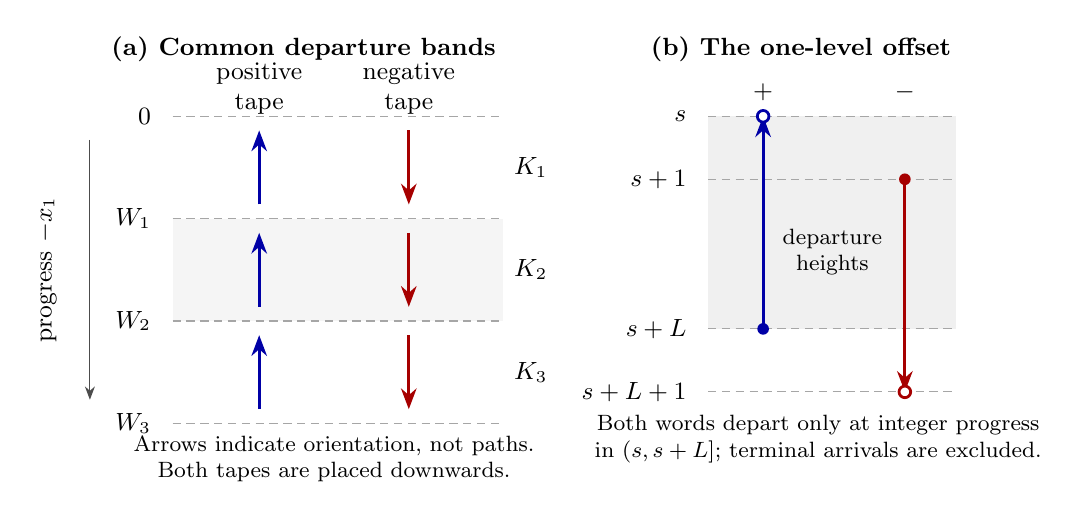
\begin{tikzpicture}[
  x=1cm,y=1cm,>=Stealth,
  every node/.style={font=\small},
  plus/.style={draw=blue!65!black,line width=1pt},
  minus/.style={draw=red!65!black,line width=1pt},
  guide/.style={draw=black!35,densely dashed,line width=.4pt}
]
  \node[anchor=west,font=\small\bfseries] at (0,.85)
    {(a) Common departure bands};
  \node[align=center] at (2.0,.35) {positive\\tape};
  \node[align=center] at (3.9,.35) {negative\\tape};
  \fill[black!4] (.9,-1.3) rectangle (5.1,-2.6);
  \foreach \yy/\lab in {0/0,-1.3/W_1,-2.6/W_2,-3.9/W_3} {
    \draw[guide] (.9,\yy)--(5.1,\yy);
    \node[anchor=east] at (.75,\yy) {$\lab$};
  }
  \foreach \top/\bottom/\j in {0/-1.3/1,-1.3/-2.6/2,-2.6/-3.9/3} {
    \draw[plus,->] (2.0,\bottom+.18)--(2.0,\top-.18);
    \draw[minus,->] (3.9,\top-.18)--(3.9,\bottom+.18);
    \node at (5.45,{(\top+\bottom)/2}) {$K_{\j}$};
  }
  \draw[->,black!70] (-.15,-.30)--(-.15,-3.60);
  \node[rotate=90,anchor=south] at (-.45,-1.95) {progress $-x_1$};
  \node[align=center,font=\footnotesize] at (2.95,-4.35)
    {Arrows indicate orientation, not paths.\\Both tapes are placed downwards.};

  \begin{scope}[xshift=7.0cm]
    \node[anchor=west,font=\small\bfseries] at (-.15,.85)
      {(b) The one-level offset};
    \node at (1.4,.30) {$+$};
    \node at (3.2,.30) {$-$};
    \fill[black!6] (.7,0) rectangle (3.85,-2.7);
    \foreach \yy/\lab in {0/s,-.8/{s+1},-2.7/{s+L},-3.5/{s+L+1}} {
      \draw[guide] (.7,\yy)--(3.85,\yy);
      \node[anchor=east] at (.55,\yy) {$\lab$};
    }
    \draw[plus,->] (1.4,-2.7)--(1.4,0);
    \draw[minus,->] (3.2,-.8)--(3.2,-3.5);
    \fill[blue!65!black] (1.4,-2.7) circle (2.1pt);
    \draw[plus,fill=white] (1.4,0) circle (2.1pt);
    \fill[red!65!black] (3.2,-.8) circle (2.1pt);
    \draw[minus,fill=white] (3.2,-3.5) circle (2.1pt);
    \node[align=center,font=\footnotesize] at (2.28,-1.72)
      {departure\\heights};
    \node[align=center,font=\footnotesize] at (2.1,-4.10)
      {Both words depart only at integer progress\\in $(s,s+L]$; terminal arrivals are excluded.};
  \end{scope}
\end{tikzpicture}

 \caption{The opposed arrangement, schematically and not to scale.
 (a) Common departure bands; arrows indicate chronological orientation,
 while placement proceeds downwards on both tapes. (b) Endpoint progress
 for a word of width $L$ preceded by total width $s$, with the one-level
 offset restored. Filled points are starts and open points are terminal
 arrivals. Word interiors and lateral positions are not depicted;
 the arrows do not assert monotonicity of the words.}
 \label{fig:arrangement}
\end{figure}
For integers $0\le a<b$, denote by $\mathcal C(a,b]$ the event
of a contact in at least one block with index $a<j\le b$.
The quantity to be estimated is
\begin{equation}\label{eq:contact-count}
 m(J)=\sum_{j=1}^J\mathbf P\bigl(\mathcal C(2^j,2^{j+1}]\bigr),
 \qquad J\ge1.
\end{equation}
It is the expected number of dyadic block-index intervals containing
a contact.  Section~\ref{sec:entropy} bounds it above using the
finite first moment of the lateral increment $S$; the remaining
sections obtain an incompatible lower bound from the forced contact
near the top and the renewal-tail estimate.

\section{An entropy upper bound for contacts}\label{sec:entropy}

We continue under the assumption that both coordinate signs have positive
probability.  The opposed arrangement and its common blocks are those of
Section~\ref{sec:arrangement}.  We will prove
\begin{proposition}\label{prop:entropy-upper}
Suppose that both coordinate signs have positive directional-transience
probability. In the opposed arrangement of Section~\ref{sec:arrangement},
let $m(J)$ be the expected number of dyadic common-block index intervals
$(2^j,2^{j+1}]$, $1\le j\le J$, containing a departure-site contact,
as in~\eqref{eq:contact-count}. Then
\[
 m(J)=O\!\left(\frac{J}{\log J}\right)\qquad(J\longrightarrow\infty).
\]
\end{proposition}
The argument compares a piece of the opposed arrangement with independent
bridges of prescribed heights.  Contacts are rare under the bridge law.
The cost of this comparison is controlled by the entropy gained when more
independent common-block displacements are added.

\subsection{A randomized comparison with independent bridges}

Fix an integer $n\ge1$.  We want to cover the common blocks with
indices in $(4n,8n]$ by a middle portion of the arrangement.  We will
surround it by two outer portions, each of height at least $n$, so
that any middle contact occurs well inside a finite slab.  A buffer
above all three portions supplies an independent lateral gap.

We randomize the number of blocks in each portion as well as in the
buffer.  Choosing a chunk count uniformly from $n$ possibilities
will offset the cost of specifying its random height.  Randomizing
the buffer count will let us compare its entropy with that of the whole
experiment without paying an additional $\log n$.
Independently of the common-block tape, choose four independent
integer counts
\begin{equation}\label{eq:entropy-count-windows}
 \begin{split}
 U,I_1,I_3&\ \hbox{uniform on }\{n,\ldots,2n-1\},\\
 I_2&\ \hbox{uniform on }\{7n,\ldots,8n-1\}.
 \end{split}
\end{equation}
Read a buffer of $U$ common blocks, followed by three chunks of
$I_1,I_2,I_3$ common blocks.  Let $d_0$ be the lateral gap after the
buffer, namely the sum of its gap increments.  For chunk $i$, let
$A_i$ and $B_i$ be the positive and negative slab lists in their
downward tape order, and let $H_i$ be their common total width.  Write
\[
 H=(H_1,H_2,H_3),\qquad
 \mathcal A=(A_1,A_2,A_3),\qquad
 \mathcal B=(B_1,B_2,B_3).
\]
The three chunks are independent, and $(U,d_0)$ is independent of all
their data.  To see this despite their random boundaries, condition
on the four external counts and use the product law of the common
blocks; the distribution of a chunk depends only on its own count.
The first and third count windows ensure the required outer heights.
The longer middle window ensures that the middle chunk starts before
block $4n$ and ends after block $8n$.

Set $q=d-1$, and let $X_{A,i},X_{B,i}\in\ZZ^q$ be the sums of the
lateral displacements of the words in $A_i,B_i$, measured in the words' actual chronological
directions.  The total positive displacement determines where its
bottom lies relative to its top.  Accordingly, define
\begin{equation}\label{eq:entropy-alignment-variables}
 X_A=\sum_{i=1}^3X_{A,i},\quad X_B=\sum_{i=1}^3X_{B,i},\quad
 Z=d_0+X_A,\quad T=U+I_1+I_2+I_3.
\end{equation}
Here is the placement that explains the alignment variable $Z$ and
will define the same contact event under the actual and reference
laws.  Set $N_*=H_1+H_2+H_3$.  Place the positive chunks
from height $0$ and lateral position $0$, in chronological order
$3,2,1$, reversing the list order within each chunk.  Each word is
still traversed in its original direction.  Place the negative chunks
in chronological order $1,2,3$ from height $N_*-1$ and lateral position
$Z$.  Let $E_{\mathrm{mid}}$ be a departure contact between the two
middle chunks.

For these actual chunk data, this placement reproduces the infinite
opposed arrangement after its buffer, up to translation.  For example,
at the top of the middle chunk the lateral gap, negative minus positive, is
\[
 Z+X_{B,1}-(X_{A,3}+X_{A,2})
   =d_0+X_{A,1}+X_{B,1},
\]
as in the original arrangement; the subsequent list placements also
agree.  From \eqref{eq:entropy-count-windows}, the middle chunk starts
after at most $4n-2$ common blocks and ends after at least $9n$ blocks.
It therefore contains the deterministic common-block interval
$(4n,8n]$.

Denote the actual law of $(H,Z,\mathcal A,\mathcal B)$ by $P_n$.
Define a reference law $Q_n$ as follows.  First sample $(H,Z)$ with its
actual joint marginal.  Given these values, sample the six lists
independently, with respective exact-cut bridge laws
$\mathcal B_{H_i}^+$ and $\mathcal B_{H_i}^-$ from
Lemma~\ref{lem:exact-bridge}.  The reference retains the dependence
between $H$ and $Z$; it changes only the conditional law of the lists.
Apply the same placement rule to its newly sampled lists.  Thus $E_{\mathrm{mid}}$ is one fixed
measurable event in both experiments, and its actual probability
bounds the original contact probability in $(4n,8n]$.

\subsection{The entropy cost of the comparison}

We use entropy and relative entropy in their classical information-theoretic
sense~\cite{Shannon1948,KullbackLeibler1951}, recalling the identities and
bounds needed for the countable path spaces below.

For a countable random variable $V$, write
\[
 \mathcal H(V)=-\sum_v P(V=v)\log P(V=v),
\]
with $0\log0=0$.  Conditional entropy is the average of the corresponding
conditional entropies.  For probability measures $P,Q$ on a countable set,
their relative entropy is
\[
 D(P\Vert Q)=\sum_x P(x)\log\frac{P(x)}{Q(x)},
\]
with value $+\infty$ if $P$ is not absolutely continuous with respect to
$Q$.  Conditional mutual information $I(V;W\mid H)$ is the average,
over $H$, of the relative entropy between the joint conditional law and
the product of its two marginals.

We use the chain rule for relative entropy, obtained by factoring joint
probabilities into marginal and conditional probabilities.  In particular,
if a reference law for $(V,W)$ conditional on $H$ factors between $V$ and
$W$, the averaged conditional relative entropy is at least
$I(V;W\mid H)$.  Nonnegativity of relative entropy follows from Jensen's
inequality applied to $-\log$.  The same factorization, followed by
nonnegativity, shows that applying a measurable map cannot increase
relative entropy.  These facts apply to countable path lists without
assuming that the lists themselves have finite entropy; equivalently one
may first use finite partitions and pass to their increasing limit.

Let $S_1,S_2,\ldots$ be the iid lateral gap increments of the common
blocks, and set
\[
 h_k=\mathcal H(S_1+\cdots+S_k),\qquad k\ge1.
\]
Lemma~\ref{lem:common-blocks} gives $\mathbf E|S_1|<\infty$.  For a
$\ZZ^q$-valued variable with finite first moment, comparison with the
probability weights proportional to $\exp(-|x|/(k+1))$ gives
\begin{equation}\label{eq:gap-entropy-growth}
 h_k\le C+q\log(k+1).
\end{equation}
Indeed the normalizing sum is at most $C_q(k+1)^q$, and the expected
comparison energy is at most $k\mathbf E|S_1|/(k+1)$.  Also $h_k$ is
nondecreasing: condition on the last independent summand, use translation
invariance of entropy, and then remove the conditioning.

By Lemma~\ref{lem:common-blocks}, the sum of the slab radii in a common
block has finite expectation.  Thus each tape's block displacement,
and not only their sum $S$, has a finite first absolute moment.  In
addition the common width has finite mean.  All count, height, and
displacement variables used below therefore have first moments of
order $n$, and their joint and conditional entropies are finite.
No entropy bound for the full path lists is needed.

\begin{lemma}\label{lem:entropy-comparison}
There is a constant $C$, independent of $n$, such that
\[
 D(P_n\Vert Q_n)\le C+h_{14n}-h_n.
\]
\end{lemma}
\begin{proof}
There are two costs to control: imposing the random chunk heights,
and then retaining the aligned starting displacement $Z$.  We first
condition on $H$ alone.  For a specified
pair of slab lists of common total width $h$, let $r$ be the number of
their common positive cumulative widths, including $h$.  The pair is
uniquely parsed into its first $r$ common blocks.  If $r$ belongs to the
count window for chunk $i$, its actual unconditioned mass is
\[
 \frac1n\prod_{a\in A_i}W(a)\prod_{b\in B_i}W(b).
\]
It has zero mass otherwise.  The independent exact-cut bridge pair at
height $h$ has mass given by the same product divided by $u_h^+u_h^-$.
Thus the conditional density of the actual pair, on its support, is
\begin{equation}\label{eq:count-window-density}
 \frac{u_h^+u_h^-}{nP_n(H_i=h)}.
\end{equation}
Common cuts here are counted in the original downward list order,
before any list is reversed for chronological placement.

Let $D_0$ be the averaged conditional relative entropy of
$(\mathcal A,\mathcal B)$ given $H$ with respect to these independent
bridges.  The chunks are independent, so \eqref{eq:count-window-density}
and $u_h^\pm\le1$ give
\[
 D_0\le\sum_{i=1}^3\bigl(\mathcal H(H_i)-\log n\bigr)\le C.
\]
For the last bound, $\mathbf E H_i\le8n\mathbf E K$, and a positive
integer variable with mean $a$ has entropy at most $1+\log(a+1)$,
by comparison with a geometric distribution.  Since the reference
conditional on $H$ factors between the tapes,
\begin{equation}\label{eq:conditional-tape-information}
 I(\mathcal A;\mathcal B\mid H)\le D_0.
\end{equation}

Introducing $Z$ while retaining its actual marginal costs precisely
its conditional mutual information with the lists.  The chain rule
and the independence of the buffer give
\begin{equation}\label{eq:endpoint-information-cost}
 \begin{split}
 D(P_n\Vert Q_n)
 &=D_0+I(Z;\mathcal A,\mathcal B\mid H)\\
 &=D_0+\mathcal H(Z\mid H)-\mathcal H(d_0).
 \end{split}
\end{equation}
Conditional on $\mathcal A,H$, the variable $Z$ is obtained by adding
the independent $d_0$.  Data processing in
\eqref{eq:conditional-tape-information} therefore yields
$I(Z;\mathcal B\mid H)\le D_0$.

The direct bound $\mathcal H(Z\mid H)=O(\log n)$ would be too
large after summing over scales.  Instead, add the negative tape's
displacement to $Z$.  Their sum is the total common-block gap, whose
entropy can be compared with that of the buffer.  Conditioning on
the negative tape costs at most $D_0$, as just proved:

\begin{align}
 \mathcal H(T,Z+X_B)
 &\ge \mathcal H(T,Z+X_B\mid\mathcal B,H)
  =\mathcal H(T,Z\mid\mathcal B,H)\notag\\
 &\ge \mathcal H(Z\mid H)-D_0
       +\mathcal H(T\mid Z,\mathcal A,\mathcal B,H)\notag\\
 &=\mathcal H(Z\mid H)-D_0+\mathcal H(U\mid d_0).
 \label{eq:buffer-entropy-chain}
\end{align}
For the last equality, the two lists in each chunk determine its common
count.  Knowing these lists and $Z$ therefore fixes both $T-U$ and
$d_0=Z-X_A$.  The buffer pair is independent of the chunks.

The vector $Z+X_B$ is the sum of the first $T$ common gap increments.
The count $T$, like $U$, is independent of the underlying iid tape;
we are not conditioning on the observed chunks in the following
identities.  Consequently
\[
 \mathcal H(T,Z+X_B)=\mathcal H(T)+\mathbf E h_T,
 \qquad
 \mathcal H(U,d_0)=\log n+\mathbf E h_U.
\]
Here $n\le U<2n$ and $10n\le T\le14n-4$, so $T$ takes at most $4n$
values.  Monotonicity of $h_k$ gives
\begin{equation}\label{eq:random-count-entropy-difference}
 \mathcal H(T,Z+X_B)-\mathcal H(U,d_0)
 \le\log4+h_{14n}-h_n.
\end{equation}
Subtract $\mathcal H(d_0)$ in \eqref{eq:buffer-entropy-chain} and use
$\mathcal H(U,d_0)=\mathcal H(d_0)+\mathcal H(U\mid d_0)$.
Together with \eqref{eq:endpoint-information-cost} and
\eqref{eq:random-count-entropy-difference}, this gives explicitly
\[
 D(P_n\Vert Q_n)\le 2D_0+\log4+h_{14n}-h_n.
\]
The bound for $D_0$ is uniform in $n$, so its doubled contribution
is absorbed into $C$.  This proves
Lemma~\ref{lem:entropy-comparison}.
\end{proof}

\subsection{Rare contacts under the reference law}

Comparing opposed paths in one environment and classifying intersection
sites by quenched escape probabilities already appears in the planar
argument of Zerner~\cite[Section~2]{Zerner2007}. We prove the finite-barrier
estimate needed here.

\begin{lemma}\label{lem:reference-contact}
For the reference experiment just defined,
\[
 Q_n(E_{\mathrm{mid}})
 \le\delta_n:=\min\{1,Cn(F_+(n)+F_-(n))\}.
\]
\end{lemma}
\begin{proof}
Fix $(H,Z)$ in its retained support; in particular $H_1,H_3\ge n$.
Write $N=N_*$.  By list-reversal invariance in
Lemma~\ref{lem:exact-bridge}, the placed chronological chunks have
their corresponding raw bridge laws.

Retain the complete positive lower and middle chunks, concatenated
into a path $\alpha$ from height $0$ to its first hit of $N-H_1$.
Retain the negative upper and middle chunks only up to their first
arrival at a departure site of $\alpha$.  A middle contact ensures
that this arrival occurs before the negative middle endpoint at
height $H_3-1$.  The contact site $y$ must therefore satisfy
\begin{equation}\label{eq:reference-contact-height}
 H_3\le y_1\le N-H_1-1.
\end{equation}
Thus each path has made at least $n$ progress in its own signed height
before reaching the contact, and neither has crossed the global
barriers $-1,N$.

We explain the comparison with two paths in one environment before
using any quenched exit probabilities.  The unused positive upper
chunk and negative lower chunk integrate to one.  The remaining four
bridge normalizations are bounded by $p_+^{-2}p_-^{-2}$.  Consecutive
bridges within a sign have disjoint departure layers, so their raw
weights multiply to the raw weight of their concatenation.  Summing
over the negative completion after its retained prefix, and dropping
its remaining bridge requirements, costs at most that prefix's raw
weight: in each fixed environment the total conditional completion
probability is at most one, and this inequality can then be averaged.
This argument allows the completion to revisit its prefix's departure
rows and does not factor their weights independently.
The first-hit chunk boundaries determine the splits, so no
extra multiplicity is introduced.

The retained negative prefix has no departure site in
$\operatorname{Dep}(\alpha)$: its terminal point is the first arrival
there.  Repeated sites within either path cause no difficulty.
Lemma~\ref{lem:departure-transfer} therefore identifies the product
of their raw weights with the weight of the two paths sampled
independently conditional on a common iid environment.  For each
$\alpha$ the first contact fixes the negative prefix uniquely, and
$\alpha$ itself is stopped at a fixed first-hit height.  We may thus
sum these joint prefix weights without overcounting, and extend the
paths as raw trajectories in the common environment.

Only now, in that shared environment, define for interior sites
\[
 Q_y^\omega=P_{y,\omega}(T_{-1}<T_N),
\]
where the barriers are absolute first-coordinate heights.  If
$Q_y^\omega\ge1/2$ at the contact, the positive raw path has visited
such a site after hitting $n$ and before exiting the global slab.
Conditional on the environment, stop it at its first such visit.
The probability of a subsequent exit at $-1$ is at least $1/2$.
Consequently the annealed probability of this visit event is at most
\[
 2P_0(T_n<T_{-1}<T_N)=2(u_n^+-u_N^+).
\]
If $Q_y^\omega<1/2$, the negative marginal gives the analogous bound
$2(u_n^--u_N^-)$.  Indeed the almost-sure finite-height-interval
exit property established in Section~\ref{sec:arrangement} holds
quenched for all these starting sites and barriers outside one
null set.  The probability of the other exit is therefore greater
than $1/2$, with no common lower bound on the transition rows.
Measured from the negative start $N-1$, the
global barriers $N$ and $-1$ have signed relative heights $-1$ and
$N$, respectively.  Lateral translation by $Z$ does not change its
annealed law.

Combining these alternatives with the bounded normalizations gives,
uniformly in $(H,Z)$,
\[
 Q_n(E_{\mathrm{mid}}\mid H,Z)
 \le C\sum_{\sigma\in\{+,-\}}(u_n^\sigma-u_N^\sigma)
 \le CN\bigl(F_+(n)+F_-(n)\bigr),
\]
where the last step is Lemma~\ref{lem:renewal-tail}.  Finally
$\mathbf E N\le12n\mathbf E K$.  Average over the retained joint
marginal of $(H,Z)$ and take the minimum with $1$.
\end{proof}

\subsection{Summing over scales}

\begin{proof}[Proof of Proposition~\ref{prop:entropy-upper}]
For $l\ge2$, take $n=2^{l-2}$ and abbreviate $\delta_l=\delta_n$.
The event $E_{\mathrm{mid}}$ contains the original contact event in
common blocks $(2^l,2^{l+1}]$.  If $\delta_l=0$, absolute continuity
from Lemma~\ref{lem:entropy-comparison} makes its actual probability
zero.  Otherwise the binary relative-entropy inequality gives
\begin{equation}\label{eq:binary-contact-entropy}
 P_n(E_{\mathrm{mid}})\log(1/\delta_l)
 \le C+h_{14n}-h_n.
\end{equation}
For completeness, applying data processing to an event with actual
and reference probabilities $a,b$ gives binary divergence
$a\log(a/b)+(1-a)\log((1-a)/(1-b))$.  It is at least
$a\log(1/b)-\log2$.  Use $b\le\delta_l$ and absorb $\log2$ into $C$.

Width integrability gives
\[
 \sum_{l\ge2}\delta_l<\infty.
\]
Among $2\le l\le J$, at most $C\sqrt J$ indices have
$\delta_l>J^{-1/2}$.  They contribute at most $C\sqrt J$ to $m(J)$.
For every other index with positive $\delta_l$, the logarithm in
\eqref{eq:binary-contact-entropy} is at least $\tfrac12\log J$.
Since $14n\le16n$, monotonicity and bounded overlap give
\[
 \sum_{l=2}^J\bigl(h_{14\cdot2^{l-2}}-h_{2^{l-2}}\bigr)
 \le\sum_{l=2}^J\bigl(h_{2^{l+2}}-h_{2^{l-2}}\bigr)
 \le4h_{2^{J+2}}=O(J),
\]
using \eqref{eq:gap-entropy-growth}.  Summing
\eqref{eq:binary-contact-entropy}, and adding the initial scale, proves
\[
 m(J)\le1+C\sqrt J+\frac{CJ}{\log J}
       =O(J/\log J).
\]
\end{proof}

The estimate uses the same departure contacts as the original
arrangement.  The next section bounds the chance of a first contact
far above a true cut; that bound will force more contact scales than
Proposition~\ref{prop:entropy-upper} permits.

\section{Contacts with a path anchored at a random endpoint}
\label{sec:posterior}

The lower contact bound requires a different comparison from the one used in
Section~\ref{sec:entropy}.  A positive bridge now determines the starting
point of the negative path.  We control this dependence by retaining the
conditional probabilities of the bridge's possible endpoints.  The needed
estimate for these probabilities is a finite-vector martingale inequality.

\subsection{The sum of posterior maxima}

The first-moment calculation integrates the nonnegative-martingale maximal
inequality, whose classical form appears in
\cite[Chapter~V, Premi\`ere section, \S2, Theorem~1]{Ville1939}.
The same coordinatewise calculation for posterior vectors appears in
Kesselheim, Molinaro, Patton, and Singla~\cite[Section~1.1]{KesselheimMolinaroPattonSingla2026}.
To obtain an exponential moment, we also control conditional future
increases and the size of each jump. This is the increasing-process
energy mechanism of~\cite[Theorem~4 and its corollary]{Kikuchi1992};
we give an elementary threshold proof with the required filtration explicit.

\begin{lemma}[Posterior maxima]\label{lem:posterior-maxima}
Let $m\ge1$, and let $(w_i(e))_{i\ge0}$, $1\le e\le m$, be nonnegative
martingales for a filtration $(\mathcal F_i)$, with
$\sum_{e=1}^m w_i(e)\le1$ almost surely.  Define
\[
 A_i(e)=\max_{0\le j\le i}w_j(e),\qquad
 A_i=\sum_{e=1}^m A_i(e).
\]
Write $A_\infty(e)=\lim_{i\to\infty}A_i(e)$ and
$A_\infty=\sum_e A_\infty(e)=\lim_{i\to\infty}A_i$.
There are absolute constants $c,C>0$ such that
\begin{equation}\label{eq:posterior-exponential}
 \EE\exp\left(\frac{cA_\infty}{\log(m+1)}\right)\le C.
\end{equation}
Moreover, if $V$ is any event on a joint probability space with this
martingale-path marginal and $p=P(V)$, then
\begin{equation}\label{eq:posterior-event-weight}
 \EE[A_\infty\1_V]
 \le C\log(m+1)\,p\log(e/p),
\end{equation}
where the right side is zero when $p=0$.  The event $V$ need not belong to
any $\mathcal F_i$.
\end{lemma}

\begin{proof}
Write $B=\log(m+1)$.  We first show that, at every almost surely finite
stopping time $\rho$,
\begin{equation}\label{eq:posterior-future-increase}
 \EE[A_\infty-A_\rho\mid\mathcal F_\rho]\le B.
\end{equation}
For a fixed coordinate put $a=A_\rho(e)$ and $p_e=w_\rho(e)$, so that
$0\le p_e\le a\le1$.  Conditional maximal inequality and integration over
levels give, when $a>0$,
\[
 \EE[A_\infty(e)-a\mid\mathcal F_\rho]
 \le\int_a^1\frac{p_e}{u}\,du
 =p_e\log(1/a)\le p_e\log(1/p_e).
\]
If $a=0$, the martingale has conditional expectation zero at every later
time and contributes zero.  The conditional maximal inequality follows
first for bounded stopping times and finite horizons; localization and
monotone convergence give the displayed version.  Summing over $e$ and
adding the missing mass $1-\sum_e p_e$ bounds the resulting sum by the
entropy of a probability vector on $m+1$ elements, hence by $B$.  This
proves~\eqref{eq:posterior-future-increase}.

At each time the increase of a coordinate maximum is at most its current
value.  Consequently
\[
 A_0\le1,\qquad 0\le A_i-A_{i-1}\le\sum_e w_i(e)\le1.
\]
Set $b=2B+1$ and consider the successive thresholds $1+kb$, $k\ge1$.
At their first strict crossings, the overshoot is at most one.  After a
crossing, reaching the next threshold requires a further increase greater
than $b-1=2B$.  Conditional Markov inequality
and~\eqref{eq:posterior-future-increase} therefore bound the conditional
probability of this next crossing by $1/2$.  The first crossing has the
same bound since $A_0\le1$.  Applying this argument at finite horizons
and then letting the horizon increase yields
\[
 P(A_\infty>1+kb)\le2^{-k}.
\]
Because $B\ge\log2$, this is an exponential tail on scale $B$, and its
integral proves~\eqref{eq:posterior-exponential}.

Finally, for $p>0$, conditional Jensen inequality gives
\[
 \exp\left(\frac{c\,\EE[A_\infty\mid V]}{B}\right)
 \le \EE[\exp(cA_\infty/B)\mid V]\le C/p.
\]
Multiplication by $p$ and an adjustment of the absolute constant give
\eqref{eq:posterior-event-weight}.  This last argument uses only a
marginal exponential moment, so it applies to events in a larger joint
space without any assertion that the martingales remain martingales in
an enlarged filtration.
\end{proof}

\subsection{A first-contact estimate}

The comparison of opposing paths through unvisited rows and the use of
quenched exit probabilities are related to Zerner's planar
argument~\cite[Section~2]{Zerner2007}. Here the negative path starts at
a random endpoint of the positive bridge; the posterior estimate controls
the dependence created by that alignment.

We continue to use integer height $x_1$, and write $\pi x\in\ZZ^{d-1}$
for the lateral coordinates of $x\in\ZZ^d$.  Recall that
$u_n^+=P_0(T_n<T_{-1})$ and $p_\pm>0$ are the non-backtracking
probabilities.  The constants below may depend on the environment law and
the dimension.  We assume only strict positivity of the transition rows;
no common ellipticity bound is imposed.

Fix an integer $N\ge3$.  Let $Y$ have the annealed bridge law from $0$ to its first
arrival at height $N$, conditioned on $T_N<T_{-1}$, and put
$E=\pi Y_{T_N}$.  Independently sample a negative path $B$ with law
$\widehat P_{-e_1}$.  Translate it to the random starting site $(N-1,E)$:
\[
 \beta_j=(N-1,E)+B_j,\qquad j\ge0.
\]
Thus the relative negative path is independent of the positive bridge;
its absolute position depends on the bridge endpoint.  A departure of
$Y$ means an index $i<T_N$.  Every site of the infinite path $\beta$ is
a departure site.  For a negative path started at height $N-1$, write
$D^-$ for the event that it never rises above $N-1$.

\begin{proposition}[First contact after a prescribed height]
\label{prop:contact-bound}
In the preceding experiment, let $0<k<r<N$ be integers and define
\[
 \tau=\inf\{i\ge T_k:i<T_N,\ Y_i\in\{\beta_j:j\ge0\}\},
 \qquad
 \Delta=u^+_{r-k}-u^+_{N-k}.
\]
An empty infimum is $+\infty$.  Then
\begin{multline}\label{eq:first-contact-bound}
 P\left(T_r\le\tau<T_N,\
       \min_{T_k\le i\le\tau}(Y_i)_1\ge k,\
       \|E\|\le N^2\right)\\
 \le C\log(2N)\,\Delta\log^2(e/\Delta),
\end{multline}
with right side zero when $\Delta=0$.
\end{proposition}

The estimate is useful when the remaining gap $N-r$ is small relative
to the height $r-k$ already crossed. Lemma~\ref{lem:renewal-tail} gives
$\Delta\le (N-r)F_+(r-k)$; Section~\ref{sec:contradiction} arranges
precisely this separation of scales.

The time $\tau$ refers to the entire negative trajectory and is not
asserted to be a stopping time for the positive path.  We will enumerate
finite prefixes to use its first-contact property.  Martingale estimates
will instead be stopped at deterministic height barriers.

\begin{proof}
Let $\mathcal E_N=\{e\in\ZZ^{d-1}:\|e\|\le N^2\}$.  Its cardinality
satisfies
\begin{equation}\label{eq:endpoint-cardinality}
 \log(|\mathcal E_N|+1)\le C_d\log(2N).
\end{equation}
We first express the event in~\eqref{eq:first-contact-bound} by raw path
weights, then transfer those weights to a shared environment, and only
afterward introduce quenched exit probabilities.

\paragraph{The lower prefix and the endpoint likelihood.}
Enumerate a word $a_0$ from $0$ to its first arrival at height $k$, before
height $-1$.  Its departure sites all have height less than $k$; write
$z$ for its terminal site.  For each $e\in\mathcal E_N$, enumerate a word
$a$ from $z$ to the first contact arrival.  The required words stay in
heights $k,\ldots,N-1$ and reach height $r$ before or at their terminal
time.  Let $\operatorname{Dep}(a)$ denote the departure sites of $a$,
excluding its terminal site unless that site occurred earlier as a
departure.

For any such positive prefix define
\[
 w(a_0a;e)=P_0\bigl(T_N<T_{-1},\ \pi X_{T_N}=e
                   \mid X\text{ begins with }a_0a\bigr).
\]
This is a deterministic function of the two words and $e$.  The two
departure sets of $a_0$ and $a$ are disjoint, so the positive prefix and
completion have raw probability
\begin{equation}\label{eq:prefix-completion-weight}
 W(a_0)W(a)w(a_0a;e).
\end{equation}
For a raw negative walk started at $(N-1,e)$, let $\mathcal B(a)$ be the
event that it never rises above $N-1$, avoids $\operatorname{Dep}(a)$
at every time, and visits the terminal site of $a$.  The first-contact
condition is exactly this avoidance and visit condition.  In particular,
if the terminal site of $a$ occurred earlier as a departure, the event
$\mathcal B(a)$ is empty.  Summing
\eqref{eq:prefix-completion-weight} times the raw probability of
$\mathcal B(a)$, over these words and endpoints, and dividing by
$u_N^+p_-$ gives the probability on the left
of~\eqref{eq:first-contact-bound}.

\paragraph{Transfer and unique prefix counting.}
For a fixed word $a$, the quenched probability of $\mathcal B(a)$ uses
no rows at $\operatorname{Dep}(a)$.  Indeed the walk can be killed on
first arrival at this set, before any row there is used.  This remains
valid for the infinite avoidance event by passage from finite paths.
The departure-row identity of Lemma~\ref{lem:departure-transfer} therefore
gives
\begin{equation}\label{eq:unclassified-lower-transfer}
 W(a)P_{(N-1,e)}(\mathcal B(a))
 =\EE\left[p_\omega(a)
       P_{(N-1,e),\omega}(\mathcal B(a))\right],
\end{equation}
where $p_\omega(a)$ is the quenched product of transition probabilities
along the word.  This identity has not been restricted by any
environment-dependent exit-probability condition.

Keep $W(a_0)$ as a scalar outside the new experiment.  In a fresh
i.i.d. environment sample a raw walk $Z$ from $z$ and a raw negative
walk from $(N-1,e)$, independently conditional on the environment.  We
call $Z$ the comparison path.  Formula~\eqref{eq:unclassified-lower-transfer}
expresses the sum over $a$ as an integral over these two full paths.
For each realized pair, at most one prefix $a$ of $Z$ satisfies the
avoidance and visit conditions: its terminal is the first point of $Z$
in the range of the entire negative path.  This proves uniqueness
pathwise, without using an optional-stopping assertion at contact.
The restrictions that $a$ stays above $k-1$ and reaches $r$ are retained
at this stage.

\paragraph{Stopped posteriors on the comparison path.}
Fix $a_0$ and consider the original raw positive law conditional on this
lower prefix.  In its natural continuation filtration, with no
environment revealed, the coordinates
\[
 w_i(e)=P_0\bigl(T_N<T_{-1},\ \pi X_{T_N}=e
             \mid a_0,\text{ continuation through time }i\bigr),
 \qquad e\in\mathcal E_N,
\]
are nonnegative martingales whose sum is at most one.  Stop them on
first arrival at height $k-1$ or $N$.  All departures up to this stop
have height at least $k$.  These rows are fresh under conditioning on
$a_0$, so the stopped continuation has precisely the same path law as
$Z$ stopped at
\[
 \sigma=T_{k-1}(Z)\wedge T_N(Z).
\]
Arrival at the lower boundary uses a row at height $k$, not a departure
row at $k-1$.  Thus the equality includes the terminal arrival, as
illustrated in Figure~\ref{fig:fresh-strip}.  The stopping time is
almost surely finite by
Lemma~\ref{lem:finite-supremum}: a path that never leaves this finite
height interval would have finite height supremum without tending to
negative height infinity.  The corresponding quenched assertion holds
for almost every environment, simultaneously for all lattice starting
sites and integer height intervals.

Use these same posterior functions on the observed prefixes of $Z$, and
freeze them at $\sigma$.  At arrival at $k-1$ their values need not be
zero: they still describe success before the original lower barrier
$-1$, and that completion may use rows affected by $a_0$.  We neither
recompute them in the fresh environment nor continue them through a
departure below $k$.  Put
\[
 M(e)=\sup_{0\le i\le\sigma}w_i(e),\qquad
 S_*=\sum_{e\in\mathcal E_N}M(e).
\]
Lemma~\ref{lem:posterior-maxima}
and~\eqref{eq:endpoint-cardinality}, applied in the path filtration of
the stopped comparison walk, imply uniformly in $a_0$ that
\begin{equation}\label{eq:comparison-event-weight}
 \EE[S_*\1_V]
 \le C\log(2N)\,P(V)\log(e/P(V))
\end{equation}
for every event $V$ on the joint space of the fresh environment and $Z$.
In particular, $\EE S_*\le C\log(2N)$.  The event-weight inequality,
rather than a martingale assertion after revealing the environment,
permits the next step.

\begin{figure}[tbp]
 \centering
 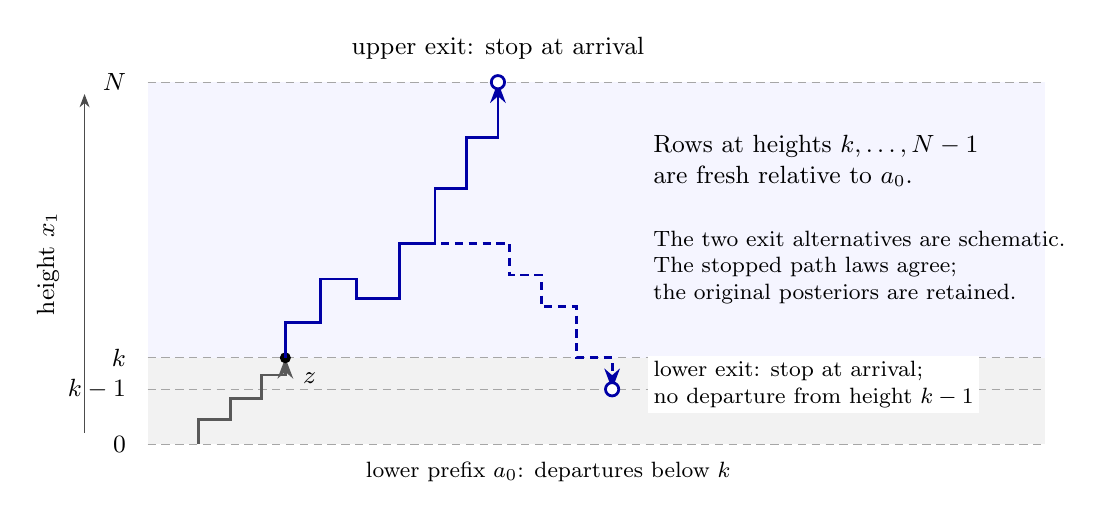
\begin{tikzpicture}[
  x=1cm,y=1cm,>=Stealth,
  every node/.style={font=\small},
  guide/.style={draw=black!35,densely dashed,line width=.4pt},
  pathline/.style={draw=blue!65!black,line width=1pt}
]
  \fill[black!5] (0,0) rectangle (11.4,1.1);
  \fill[blue!4] (0,1.1) rectangle (11.4,4.6);
  \foreach \yy/\lab in {0/{0},.7/{k-1},1.1/{k},4.6/{N}} {
    \draw[guide] (0,\yy)--(11.4,\yy);
    \node[anchor=east] at (-.15,\yy) {$\lab$};
  }
  \draw[->,black!70] (-.8,.15)--(-.8,4.45);
  \node[rotate=90,anchor=south] at (-1.0,2.3) {height $x_1$};

  \draw[black!65,line width=1pt,->]
    (.65,0)--(.65,.32)--(1.05,.32)--(1.05,.58)
    --(1.45,.58)--(1.45,.88)--(1.75,.88)--(1.75,1.1);
  \fill (1.75,1.1) circle (2pt);
  \node[anchor=north west] at (1.85,1.04) {$z$};
  \node[anchor=west,font=\footnotesize] at (2.65,-.35)
    {lower prefix $a_0$: departures below $k$};

  \draw[pathline,->]
    (1.75,1.1)--(1.75,1.55)--(2.2,1.55)--(2.2,2.1)
    --(2.65,2.1)--(2.65,1.85)--(3.2,1.85)--(3.2,2.55)
    --(3.65,2.55)--(3.65,3.25)--(4.05,3.25)--(4.05,3.9)
    --(4.45,3.9)--(4.45,4.6);
  \draw[pathline,fill=white] (4.45,4.6) circle (2.4pt);
  \node[anchor=south] at (4.45,4.77) {upper exit: stop at arrival};

  \draw[pathline,densely dashed,->]
    (3.2,2.55)--(4.6,2.55)--(4.6,2.15)--(5.0,2.15)
    --(5.0,1.75)--(5.45,1.75)--(5.45,1.1)--(5.9,1.1)
    --(5.9,.7);
  \draw[pathline,fill=white] (5.9,.7) circle (2.4pt);
  \node[anchor=west,align=left,font=\footnotesize,fill=white,inner sep=2pt] at (6.35,.76)
    {lower exit: stop at arrival;\\no departure from height $k-1$};

  \node[anchor=west,align=left] at (6.3,3.6)
    {Rows at heights $k,\ldots,N-1$\\are fresh relative to $a_0$.};
  \node[anchor=west,align=left,font=\footnotesize] at (6.3,2.25)
    {The two exit alternatives are schematic.\\The stopped path laws agree;\\the original posteriors are retained.};
\end{tikzpicture}

 \caption{Fresh rows for the stopped comparison path. The lower prefix
 first reaches height $k$ at $z$, and all its departure rows lie below
 $k$. The continuation, shown with two schematic exit alternatives,
 stops on arrival at height $k-1$ or $N$. It has used only rows with
 heights $k,\ldots,N-1$, so its stopped path law agrees with the fresh
 comparison law. The original endpoint posteriors are frozen at this
 stop, not recomputed under a new completion law. Lateral positions
 are schematic.}
 \label{fig:fresh-strip}
\end{figure}

\paragraph{Quenched exit-probability bins.}
For $k\le y_1<N$ define
\[
 Q_y^\omega=P_{y,\omega}(T_{k-1}<T_N).
\]
Almost surely every transition at every site is strictly positive.
For each interior site $y$, a finite sequence of downward axial steps
reaches $k-1$ before $N$ with positive quenched probability; a finite
sequence of upward axial steps reaches $N$ before $k-1$ with positive
quenched probability.  Thus $0<Q_y^\omega<1$, without a common bound
away from either endpoint.  Partition these values into dyadic bins
$[a,2a)$, where $a=2^{-j}$ and $j\ge1$, and write
$\mathcal D_a^\omega=\{y:k\le y_1<N,\ a\le Q_y^\omega<2a\}$
for the sites in one bin.
Let $V_a$ be the event that, at or after its first arrival at height
$r$ and before $\sigma$, the comparison path visits an interior site with
$Q_y^\omega\ge a$.  With the environment fixed, stop at the first such
visit.  The quenched Markov property gives
\begin{align}
 aP(V_a)
 &\le P_z(T_r<T_{k-1}<T_N)\notag\\
 &=u^+_{r-k}-u^+_{N-k}=\Delta.
 \label{eq:comparison-bin-probability}
\end{align}
The equality follows from nested first-hit events and almost sure exit
from the height interval, again by Lemma~\ref{lem:finite-supremum}.
These events use the fresh comparison law, not the law conditioned on
the lower prefix.

For almost every environment, the raw negative walk has probability at
most $2a$ of both satisfying $D^-$ and hitting $\mathcal D_a^\omega$.
To see this, take its first visit to that set.  On $D^-$ the negative walk
has finite first-coordinate supremum, so Lemma~\ref{lem:finite-supremum} implies that its
first coordinate tends to $-\infty$.  The quenched form of that lemma
holds outside a single environment-null set for all lattice starting
sites.  Consequently, after that first bin visit it must hit $k-1$
before $N$, even if it had previously visited $k-1$.  Its conditional
probability is at most $Q_y^\omega<2a$ by the quenched Markov property.

We now use the unique prefix established above.  In the transferred
integral, classify its contact site by its $Q^\omega$ bin and bound its
endpoint factor $w(a_0a;e)$ by $M(e)$.  Dropping the exact-contact
condition leaves $V_a$ for the comparison path and
$D^-\cap\{\hbox{the negative path hits }\mathcal D_a^\omega\}$
for the negative path.  There is no sum over competing prefixes.
After integrating the negative path, every endpoint $e$ leaves the same
fresh joint marginal $\PP(d\omega)P_{z,\omega}(dZ)$.  Thus the bin's
total contribution, summed over endpoints, is at most
\begin{equation}\label{eq:bin-contribution}
 \begin{split}
 &\sum_{e\in\mathcal E_N}\EE\left[
     M(e)\1_{V_a}
     P_{(N-1,e),\omega}
     (D^-\cap\{\hbox{the path hits }\mathcal D_a^\omega\})\right]\\
 &\hspace{35mm}\le 2a\,\EE\left[\1_{V_a}\sum_{e\in\mathcal E_N}M(e)\right]
  =2a\,\EE[S_*\1_{V_a}].
 \end{split}
\end{equation}

If $\Delta=0$, every $V_a$ is null
by~\eqref{eq:comparison-bin-probability}, proving the required zero
bound.  Suppose $\Delta>0$.  For $a<\Delta$, sum
\eqref{eq:bin-contribution} using $\EE S_*\le C\log(2N)$ and
$\sum_{a<\Delta}a\le2\Delta$.  For $a\ge\Delta$, use
\eqref{eq:comparison-event-weight} and
$P(V_a)\le\Delta/a$ to bound the contribution by
\[
 C\log(2N)\,\Delta\log(ea/\Delta).
\]
There are $O(\log(e/\Delta))$ such dyadic bins, and their logarithms
sum to $O(\log^2(e/\Delta))$.  Thus, for each fixed $a_0$, all endpoint
and upper-prefix contributions together are at most
\[
 C\log(2N)\,\Delta\log^2(e/\Delta).
\]
Finally $\sum_{a_0}W(a_0)=u_k^+\le1$, and
$1/(u_N^+p_-)\le1/(p_+p_-)$.  Restoring these factors proves
\eqref{eq:first-contact-bound}.  The constants lose only these fixed
non-backtracking probabilities and the endpoint-cardinality factor.
In particular, the argument has not required a lower bound for
$Q_y^\omega$ or an inverse-transition moment.
\end{proof}

The estimate controls a contact anywhere after the prescribed height
$r$.  It therefore applies to a long interval without subdividing the
positive path by its successive record heights.  In the next section a
missing interval of contact depths forces exactly such a late first
contact.

\section{Many contact scales and the contradiction}
\label{sec:contradiction}

We now apply Proposition~\ref{prop:contact-bound} to the opposed
arrangement.  An interval of depths containing no contact forces the first
contact above each positive cut in that interval to occur close to the
top.  The first-contact estimate makes this unlikely on average over the
cuts.  We first count scales of \emph{depth}; the finite mean common-block
width will then convert this count into the block-index count used in
Proposition~\ref{prop:entropy-upper}.

\begin{proposition}\label{prop:contact-lower}
Suppose that both coordinate signs have positive directional-transience
probability.  In the opposed arrangement of
Section~\ref{sec:arrangement}, let $m(J)$ be the expected number of
dyadic common-block index intervals $(2^j,2^{j+1}]$, $1\le j\le J$,
containing a departure-site contact, as in~\eqref{eq:contact-count}.
There are constants $c>0$ and $J_0<\infty$ such that
\[
 m(J)\ge \frac{cJ}{\log\log(3+J)}\qquad(J\ge J_0).
\]
\end{proposition}

\begin{proof}
All constants below may depend on the two slab laws.  Choose a large
integer $J$ and put
\begin{equation}\label{eq:lower-parameters}
 N=2^{2J},\qquad
 G=\left\lceil4\log_2\log(2+J)\right\rceil+3.
\end{equation}
For sufficiently large $J$, we have $3\le G<J$.  Depth means distance
below the initial top of the arrangement.
The choice $2^{-G}=O((\log J)^{-4})$ compensates for the logarithmic
losses below, while $G=O(\log\log J)$ leaves enough contact scales.

\paragraph{A bridge ending at a prescribed depth.}
Let $\mathcal C_N$ be the event that the positive tape has a cut at
depth $N$, and write
\[
 \mathbf Q_N=\mathbf P(\,\cdot\mid\mathcal C_N).
\]
The renewal identity gives
$\mathbf P(\mathcal C_N)=u_N^+\ge p_+>0$.
Under $\mathbf Q_N$, reverse the list of positive slabs through this cut
and translate its bottom to the origin.  Call the resulting chronological
path $Y$, and let $T_a$ denote its first hit of height $a$.
Lemma~\ref{lem:exact-bridge} says that $Y$ has law
$P_0(\,\cdot\mid T_N<T_{-1})$, stopped at $T_N$.
The steps within each slab retain their original order.  Denote the
lateral endpoint by $E$, so that the endpoint is $(N,E)$.  The negative
trajectory starts at $(N-1,E)$ and, relative to that starting point,
has the independent law $\widehat P_{-e_1}$.

The endpoint has a useful elementary tail bound.  On $\mathcal C_N$
there are at most $N$ positive slabs before depth $N$, since their
widths are positive integers.  The norm of their total lateral
displacement is at most the sum of their radii, hence at most the sum
of the first $N$ positive tape radii.  Proposition~\ref{prop:radius}
and Markov's inequality give
\begin{equation}\label{eq:lower-endpoint-tail}
 \EE_{\mathbf Q_N}|E|
 \le \frac{N E_+R}{p_+},
 \qquad
 \mathbf Q_N\{|E|>N^2\}\le \frac{C}{N}.
\end{equation}
This uses a spatial radius moment only.

\paragraph{An uncovered scale forces a late first contact.}
Call $l\ge0$ a contact depth label if a contact occurs at some integer
depth in $[2^l,2^{l+1})$.  For $G<l\le J$, let $U_l$ be the event
that none of the labels $l-G,l-G+1,\ldots,l$ is a contact depth label.
Equivalently, there is no contact at depths in
$[2^{l-G},2^{l+1})$.

Fix a positive cut depth
\[
 s\in I_l:=\bigl[2^l,\tfrac32\,2^l\bigr]\cap\ZZ,
 \qquad k=N-s.
\]
After the list reversal, this cut occurs at the bridge's first hit
$T_k$, and the remaining bridge stays at or above height $k$.
Indeed, every earlier slab has departure heights below $k$, while
every later slab has departure heights at least $k$.  This is a
property of the words, without a stopping-time assertion about the
cut.

There is a contact after $T_k$ and before $T_N$: the last positive
departure is $(N-1,E)$, the starting departure site of the negative
trajectory.  Let $\tau$ be the first contact since $T_k$, defined
pathwise against the entire negative trajectory.  Its depth is at
most $s<2^{l+1}$.  On $U_l$, it must therefore be strictly less than
$2^{l-G}$.  With
\[
 r=N-2^{l-G},
\]
the nearest-neighbor path must have reached height $r$ before this
contact.  Thus
\begin{equation}\label{eq:uncovered-first-contact}
 T_r\le\tau<T_N,
 \qquad Y_n\cdot e_1\ge k\quad(T_k\le n\le\tau).
\end{equation}
No restriction on drawdowns from the running maximum is needed.

For each \emph{deterministic} $s\in I_l$, let $\mathcal A_{l,s}$ be
the event in~\eqref{eq:uncovered-first-contact}, together with
$|E|\le N^2$, whether or not $s$ is a cut.  Proposition~
\ref{prop:contact-bound}, with upper stopping height $N$, applies
to this event.  Its width-probability difference satisfies
\begin{align}
 \Delta_{l,s}
 &=u^+_{s-2^{l-G}}-u^+_s\notag\\
 &\le 2^{l-G}F_+(s-2^{l-G})
 \le 2^{-G}a_l,
 \qquad a_l:=2^l F_+(2^{l-1}),
 \label{eq:lower-delta}
\end{align}
because $s-2^{l-G}\ge2^{l-1}$ and
Lemma~\ref{lem:renewal-tail} applies.  The same Lemma gives
\begin{equation}\label{eq:lower-summable-tail}
 A:=\sum_{l\ge1}a_l<\infty.
\end{equation}
Writing $\phi(x)=x\log^2(e/x)$ for $0<x\le1$ and $\phi(0)=0$,
the first-contact estimate is
\begin{equation}\label{eq:lower-fixed-cut-bound}
 \mathbf Q_N(\mathcal A_{l,s})
 \le C\log(2N)\,\phi(\Delta_{l,s}).
\end{equation}

\paragraph{Averaging over the cuts.}
Let $\mu_+=E_+L$.  The renewal-count strong law yields, almost surely
under the positive tape law,
\[
 \#\{\hbox{positive cuts in }I_l\}
 =\frac{2^{l-1}}{\mu_+}+o(2^l)
 \qquad(l\longrightarrow\infty).
\]
Fix $c_0=1/(4\mu_+)$, and let $\mathcal B_J$ be the event that
each interval $I_l$, $G<l\le J$, contains at least $c_0 2^l$
positive cuts.  Since $G=G(J)\to\infty$, the eventual almost-sure
estimate implies $\mathbf P(\mathcal B_J^c)=o(1)$.  Moreover,
\begin{equation}\label{eq:cut-density-conditioning}
 \mathbf Q_N(\mathcal B_J^c)
 \le \frac{\mathbf P(\mathcal B_J^c)}{p_+}=o(1).
\end{equation}
In particular, no independence between the cut at $N$ and the density
event is required.

On $\mathcal B_J\cap\{|E|\le N^2\}$, every uncovered label $l$
produces $\mathcal A_{l,s}$ for each actual cut $s\in I_l$.
Consequently,
\begin{equation}\label{eq:cut-averaging}
 \1_{U_l}\1_{\mathcal B_J}\1_{\{|E|\le N^2\}}
 \le \frac1{c_0 2^l}\sum_{s\in I_l}\1_{\mathcal A_{l,s}}.
\end{equation}
The right side has dropped the cut requirement on $s$.  This permits
the deterministic-barrier estimate~\eqref{eq:lower-fixed-cut-bound};
the number of summands is $O(2^l)$ and cancels the averaging factor.

We next check that the logarithms in this estimate do not require a
quantitative tail rate.  For $J\ge3$, put
\[
 B_J=\sum_{l=1}^J a_l\log_+^2(1/a_l),
 \qquad \log_+x:=\max\{\log x,0\},
\]
where a zero summand is interpreted as zero.  Terms with
$a_l\ge J^{-2}$ contribute at most $4A\log^2 J$.  On
$(0,J^{-2})$, the function $x\log^2(1/x)$ is increasing, so the
remaining at most $J$ terms contribute at most $4J^{-1}\log^2 J$.
Therefore
\begin{equation}\label{eq:weighted-tail-log}
 B_J\le 4(A+J^{-1})\log^2 J.
\end{equation}

For sufficiently large $J$, $2^{-G}a_l\le e^{-1}$ uniformly in
$l$, since $a_l\le A$.  The function $\phi$ is increasing on
$[0,e^{-1}]$.  Thus~\eqref{eq:lower-delta} gives, uniformly over
$s\in I_l$,
\[
 \phi(\Delta_{l,s})\le C2^{-G}a_l
 \bigl(G+1+\log_+(1/a_l)\bigr)^2.
\]
Taking expectations in~\eqref{eq:cut-averaging}, then using
\eqref{eq:lower-endpoint-tail},
\eqref{eq:lower-fixed-cut-bound}, and
\eqref{eq:cut-density-conditioning}, gives
\begin{align}
 \sum_{l=G+1}^J\mathbf Q_N(U_l)
 &\le J\mathbf Q_N(\mathcal B_J^c)+\frac{CJ}{N}
   +C\log(2N)\,2^{-G}\bigl[A(G+1)^2+B_J\bigr]\notag\\
 &=o(J).
 \label{eq:few-uncovered}
\end{align}
Indeed, $\log(2N)=O(J)$, while the choice~
\eqref{eq:lower-parameters} gives
$2^{-G}=O(\log^{-4}(2+J))$.  By~\eqref{eq:weighted-tail-log},
the last term is $O(J/\log^2(2+J))$.

\paragraph{Removing the conditioning.}
Let $H_J$ count contact depth labels in $\{1,\ldots,J\}$.
Equation~\eqref{eq:few-uncovered} and Markov's inequality imply
that with $\mathbf Q_N$-probability tending to one, at most $J/4$
of the tested labels are uncovered.  Since $G=o(J)$, at least
$J/2$ are then covered.  A single contact depth label $h$ can cover
only the labels $h,h+1,\ldots,h+G$.  Hence
\begin{equation}\label{eq:height-count-conditioned}
 \mathbf Q_N\left\{H_J\ge\frac{J}{2(G+1)}\right\}
 \longrightarrow1.
\end{equation}
For large $J$, all depths counted here are less than $2^{J+1}<N$.
On $\mathcal C_N$ they are therefore fully represented in the
positive list ending at depth $N$.  Undoing the translation and list
reversal leaves exactly the contacts in the original opposed
arrangement.  Thus~\eqref{eq:height-count-conditioned} implies
\begin{equation}\label{eq:height-count-unconditioned}
 \mathbf P\left\{H_J\ge\frac{J}{2(G+1)}\right\}
 \ge p_+-o(1).
\end{equation}
Only a probability bounded away from zero is asserted after removing
the conditioning.  This is enough for an expectation lower bound.

\paragraph{From depths to common-block indices.}
Write $K_1,K_2,\ldots$ for the common-block widths and
$W_i=K_1+\cdots+K_i$, with $W_0=0$.  By
Lemma~\ref{lem:common-blocks}, $\mu:=\mathbf E K_1<\infty$ and
$W_i/i\to\mu$ almost surely.  In particular, eventually
\[
 \frac\mu2 i\le W_i\le2\mu i.
\]
An integer depth $z\ge1$ belongs to the unique block
\[
 i(z)=\min\{i\ge1:W_i\ge z\},
 \qquad W_{i(z)-1}<z\le W_{i(z)}.
\]
The departure-height convention makes this true even at a common
cut depth.  For every sufficiently large $z$, the strong-law bounds
give
\begin{equation}\label{eq:depth-index-comparison}
 \frac{z}{2\mu}\le i(z)<\frac{2z}{\mu}+1.
\end{equation}
The finite initial blocks, however large their widths, disappear once
$z$ exceeds their cumulative width.

Define the dyadic index label of a block $i>1$ by
$j(i)=\lceil\log_2 i\rceil-1$, so that
$2^{j(i)}<i\le2^{j(i)+1}$.  It follows from
\eqref{eq:depth-index-comparison} that there is a deterministic
integer $c_1$, depending only on $\mu$, such that eventually
\begin{equation}\label{eq:bounded-label-shift}
 |j(i(z))-l|\le c_1
 \quad\hbox{whenever }2^l\le z<2^{l+1}.
\end{equation}
Almost surely this holds above a finite random depth.  Therefore
the probability that it holds for every contact with
$\lceil\sqrt J\rceil\le l\le J$ tends to one.

Intersect this event with the event in
\eqref{eq:height-count-unconditioned}.  The intersection still has
probability at least $p_+-o(1)$.  Discarding the first
$\lceil\sqrt J\rceil$ depth labels loses
$o(J/(G+1))$ labels.  Each remaining contact depth label supplies a
contact block whose index label lies within $c_1$ of it.  Conversely,
one index label can account for at most $2c_1+1$ depth labels.
Thus, on the intersection, at least $c_2J/(G+1)$ of the index labels
$1,\ldots,J+c_1$ contain a contact, for a fixed $c_2>0$ and large
$J$.  Taking expectations yields
\[
 m(J+c_1)\ge\frac{c_3J}{G+1}.
\]
Since $G+1=O(\log\log(3+J))$, replacing $J+c_1$ by the argument
of $m$ proves the proposition.
\end{proof}

\begin{proof}[Proof of Theorem~\ref{thm:main}]
Fix any nonzero real direction $\ell$.  Suppose that
$0<P_0(A_\ell)<1$.  Lemma~\ref{lem:sign-union} implies that
$P_0(A_{-\ell})>0$.  The spatial-radius estimate and
Proposition~\ref{prop:coordinate-reduction} then supply a coordinate
direction in which both signs have positive probability.  Reflecting
and relabeling that coordinate gives the setting of
Propositions~\ref{prop:entropy-upper} and~\ref{prop:contact-lower}.
They imply simultaneously
\[
 m(J)=O\!\left(\frac{J}{\log J}\right)
 \quad\hbox{and}\quad
 m(J)\ge\frac{cJ}{\log\log(3+J)}
\]
for all sufficiently large $J$, which is impossible.  Thus
$P_0(A_\ell)\in\{0,1\}$.

The reduction applies to every fixed real $\ell$ without rational
approximation.  Strict ellipticity supplied the fresh-row probabilities;
the spatial-radius moment was derived under coexistence.  Neither a
moment of a slab's duration nor a speed assumption entered the argument.
\end{proof}

\bibliographystyle{plain}
\bibliography{refs}
\end{document}
